\chapter{E-Government Development Index}
\label{egdi}

\cite{martinez2022egovernment} anuncia 4 tipos de índices de governo eletrônico: EGDI da ONU, GTMI do Banco Mundial, DESI da Comissão Europeia da União Europeia e DGI da OECD.

A não escolha do DESI foi motivada, principalmente, pelo seu escopo. Conforme \cite{desi_2022} explica, o índice é administrado pela Comissão Europeia e foca na análise individual de cada Estado-membro para identificar áreas prioritárias.

Como os foco da análise é o Brasil, o fato do DESI ter sua abrangência limitada a União Europeia afastou a possibilidade de seu uso. Contrariamente, o EGDI, GTMI e DGI têm abrangência global.

Escolheu-se qual índice usar pela quantidade de resultados retornados no Google Acadêmico. A figura mostra a distribuição dos resultados.

\begin{figure}[H]
	\centering
	\caption{Distribuição da quantidade de buscas encontradas dos EGDI, GTMI e DGI}
	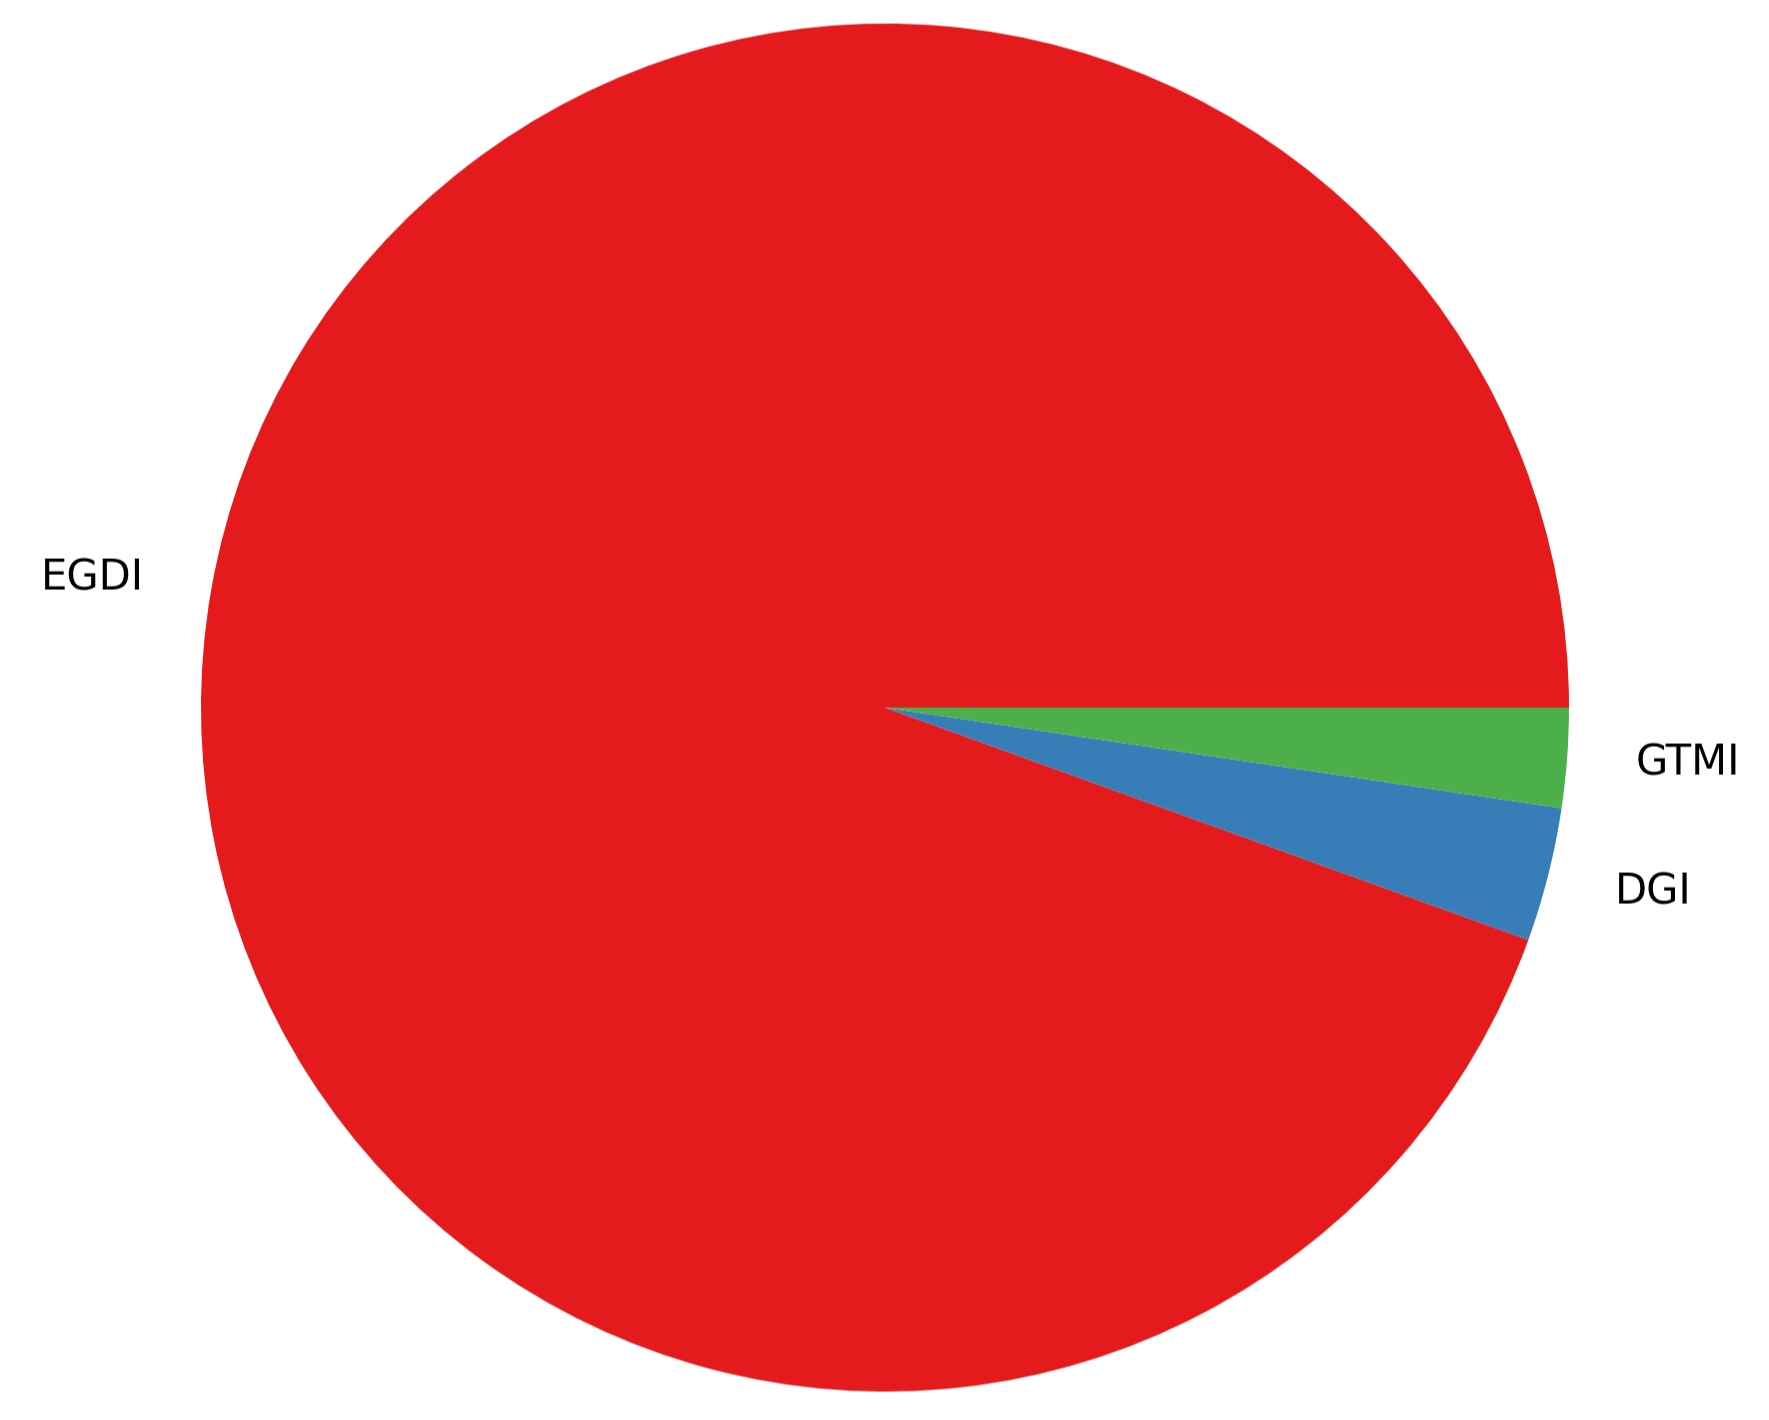
\includegraphics[width=0.6\linewidth]{figuras/indices/indices_google_academico}
	\label{fig:indices_google_academico}
	\\ \footnotesize{Fonte: elaboração própia.}
\end{figure}

Dentre os índices com abrangência global – EGDI, GTMI e DGI – optou-se pelo primeiro. Embora o GTMI do Banco Mundial e o DGI da OECD também ofereçam visões valiosas sobre a maturidade do governo digital, o EGDI da ONU foi o escolhido devido a maior quantidade de material .

O EGDI apresenta o estado de desenvolvimento de governo eletrônico dos Estados membros da ONU. O índice incorpora as características de acesso, tais como níveis de infraestrutura e educacional para mostrar como um país está usando as tecnologias de informação para promover acesso e inclusão do seu povo \cite{ONU_EGDI}.

\cite{ONU_EGDI} afirma que o EGDI é uma mensuração composta formada por 3 importantes dimensões do governo eletrônico: provisão de serviços online, conectividade de telecomunicação e capacidade humana.

Os componentes do EGDI são:

\begin{figure}[H]
	\centering
	\caption{Os três componentes do EGDI}
	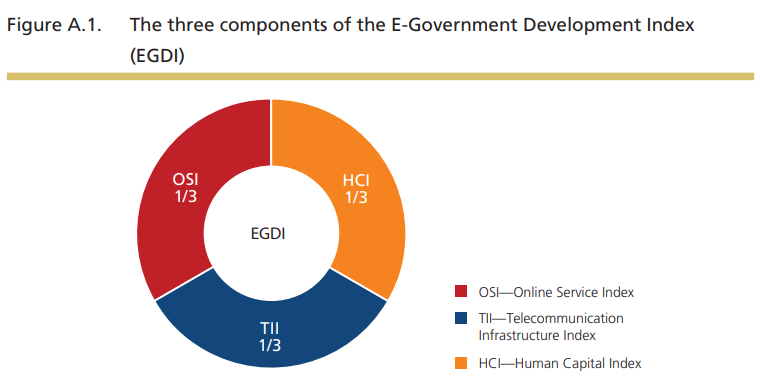
\includegraphics[width=1\linewidth]{figuras/egdi/egdi_componentes.png}
	\label{fig:egdi_componentes}
	\footnotesize{Fonte: \cite{ONU_EGDI_methodology}}
\end{figure}

A figura \ref{fig:boxplot_egov_global} contém um diagrama de caixa que representa o EGDI global.

\begin{figure}[H]
	\centering
	\caption{E-Government Development Index global em 2024}
	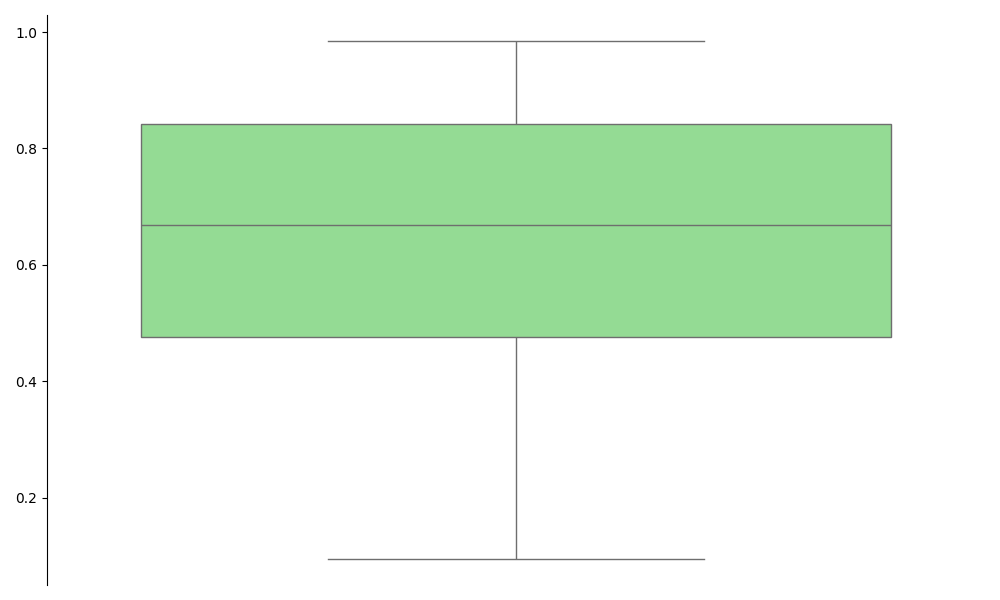
\includegraphics[width=1\linewidth]{figuras/egdi/boxplot_egov_global.png}
	\label{fig:boxplot_egov_global}
	\footnotesize{Fonte: baseado em \cite{ONU_EGDI_mapa}.}
\end{figure}

Os valores mínimo e máximo são, respectivamente, 0.09 e 0.98. O  valor médio é 0.67. Os 1º e 3º quartis são, respectivamente, 0.48 e 0.84.

\section{E-Participation Index}
\label{epart}

\cite{ONU_EGDI} argumenta que o \textbf{E-Participation Index} deriva do EGDI como índice suplementar ao relatório \textbf{E-Government Survey}. Os componentes do índice são: \textbf{E-information}, \textbf{E-consultation} e \textbf{E-decision-making}. 

\textbf{E-information} fala sobre a facilitação da participação dos cidadãos via informações públicas e acesso a informação sem necessidade de pedido ou sob demanda. \textbf{E-consultation} diz respeito ao engajamento dos cidadãos em contribuições e deliberações sobre políticas publicas e serviços públicos. \textbf{E-decision-making} engloba o empoderamento dos cidadãos via a opção de coparticipação na elaboração de políticas e coprodução de componentes de serviços e entrega de modalidades.

\cite{ONU_EGDI} esclarece que o \textbf{E-Participation Index} de um país reflete os mecanismos do índice que são empregados pelo governo quando se faz comparações com todos outros países. 

O propósito dessa medição não é prescrever qualquer prática especificam, no entanto oferece perspectivas de como países diferentes estão usando ferramentas online para promover interação entre o governo e seu povo, bem como, entre as pessoas para benefícios de todos.

A figura \ref{fig:boxplot_epart_global} contém um diagrama de caixa que representa o \textbf{E-Participation Index} global.

\begin{figure}[H]
	\centering
	\caption{E-Participation Index global em 2024}
	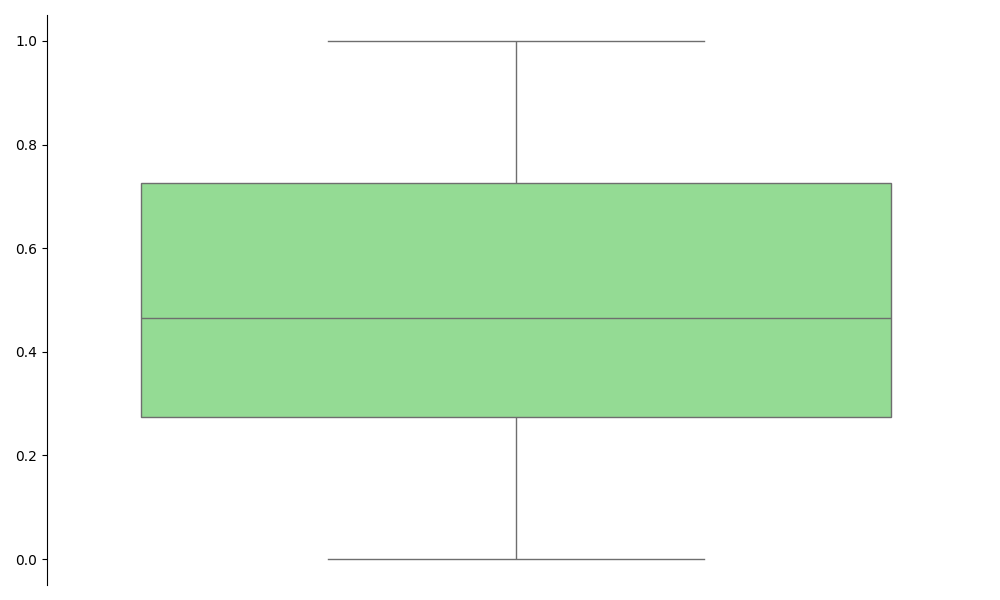
\includegraphics[width=1\linewidth]{figuras/egdi/boxplot_epart_global.png}
	\label{fig:boxplot_epart_global}
	\footnotesize{Fonte: baseado em \cite{ONU_EGDI_mapa}.}
\end{figure}

Os valores mínimo e máximo são, respectivamente, 0.0 e 1.0. O  valor médio é 0.47. Os 1º e 3º quartis são, respectivamente, 0.27 e 0.73.

\section{Online Service Index}
\label{osi}

A figura \ref{fig:boxplot_osi_global} contém um diagrama de caixa que representa o \textbf{E-Participation Index} global.

\begin{figure}[H]
	\centering
	\caption{Online Service Index global em 2024}
	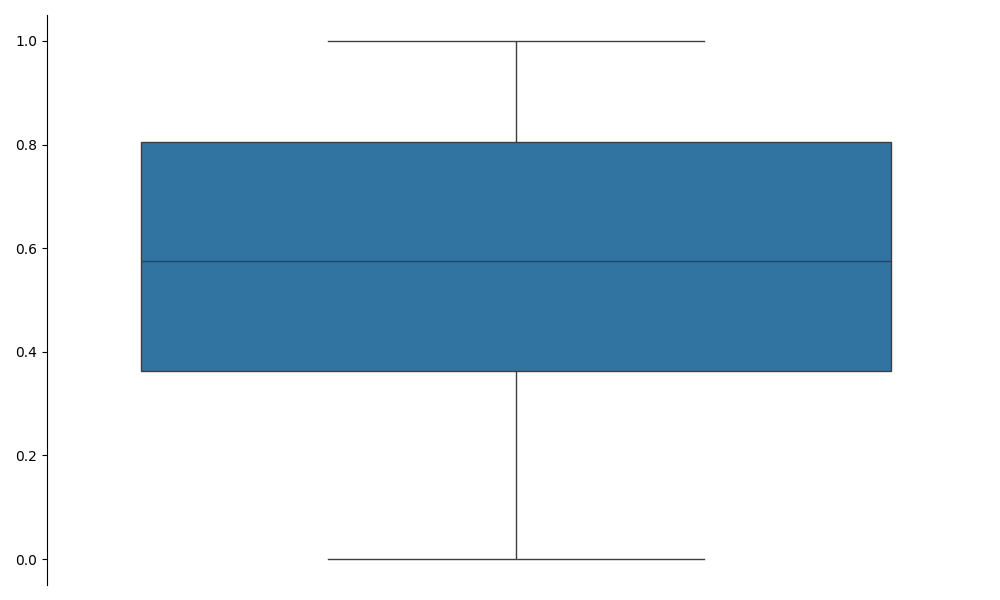
\includegraphics[width=1\linewidth]{figuras/egdi/boxplot_osi_global.png}
	\label{fig:boxplot_osi_global}
	\footnotesize{Fonte: baseado em \cite{ONU_EGDI_mapa}.}
\end{figure}

Os valores mínimo e máximo são, respectivamente, 0.0 e 1.0. O  valor médio é 0.58. Os 1º e 3º quartis são, respectivamente, 0.36 e 0.81.

\section{Human Capital Index em 2024}
\label{hci}

\cite{ONU_EGDI_methodology} afirma que \textbf{Human Capital Index} tem 4 indicadores: taxa bruta de matrícula, letramento adulto, anos de escolarização esperados e média de anos de escolaridade. 

A taxa bruta de matrícula é medida como a combinação entre a taxa de matrícula nas educações primárias, secundários e terciárias. Letramento adulto é medido como o percentual de pessoas com pelos menos 15 anos de idade que entendem e sabem ler e escrever um frase curta simples na sua vida padrão.

Os anos de escolarização esperados é o número total de anos de escolarização que crianças de certa idade podem esperar ter no futuro, presumindo que a probabilidade de a criança de qualquer idade estiver na escola correspondendo à idade da taxa de matrícula atual.

A média de anos de escolaridade fornece o número médio de anos de educação concluídos pela população adulta de um país (25 anos ou mais), excluindo os anos gastos repetindo séries. 

A figura \ref{fig:boxplot_hci_global} contém um diagrama de caixa que representa o \textbf{E-Participation Index} global.

\begin{figure}[H]
	\centering
	\caption{Human Capital Index global em 2024}
	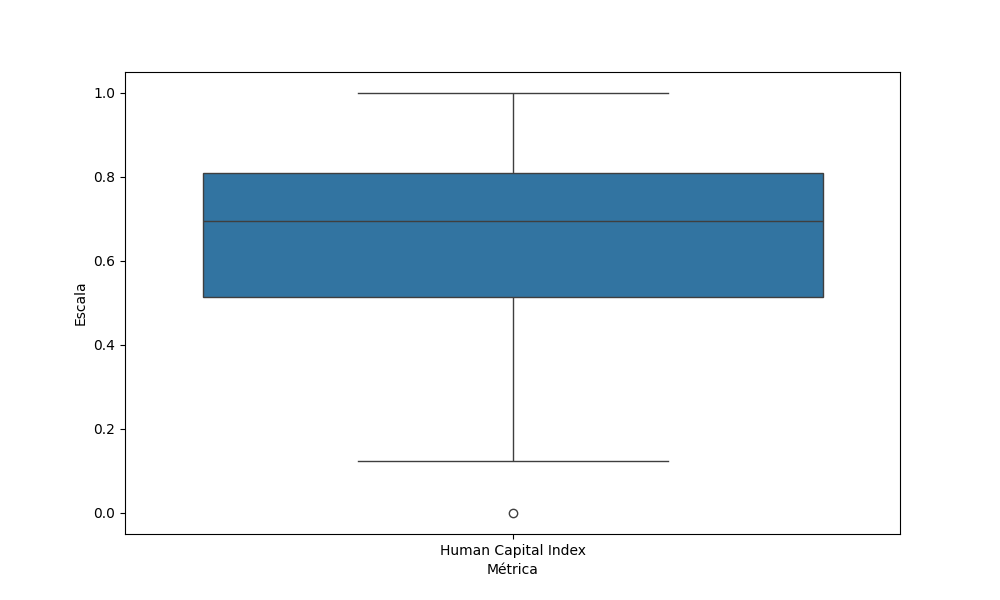
\includegraphics[width=1\linewidth]{figuras/egdi/boxplot_hci_global.png}
	\label{fig:boxplot_hci_global}
	\footnotesize{Fonte: baseado em \cite{ONU_EGDI_mapa}.}
\end{figure}

Os valores mínimo e máximo são, respectivamente, 0.0 e 1.0. O  valor médio é 0.7. Os 1º e 3º quartis são, respectivamente, 0.51 e 0.81.

\section{Telecommunication Infrastructure Index em 2024}
\label{tii}

\cite{ONU_EGDI_methodology} afirma que o \textbf{Telecommunication Infrastructure Index} tem 5 componentes: usuário de internet, assinatura de banda larga fixa, assinatura de banda larga sem fio, assinatura de telefone fixo e assinatura de dados móveis.

A figura \ref{fig:boxplot_tci_global} contém um diagrama de caixa que representa o \textbf{E-Participation Index} global.

\begin{figure}[H]
	\centering
	\caption{Telecommunication Infrastructure Index global em 2024}
	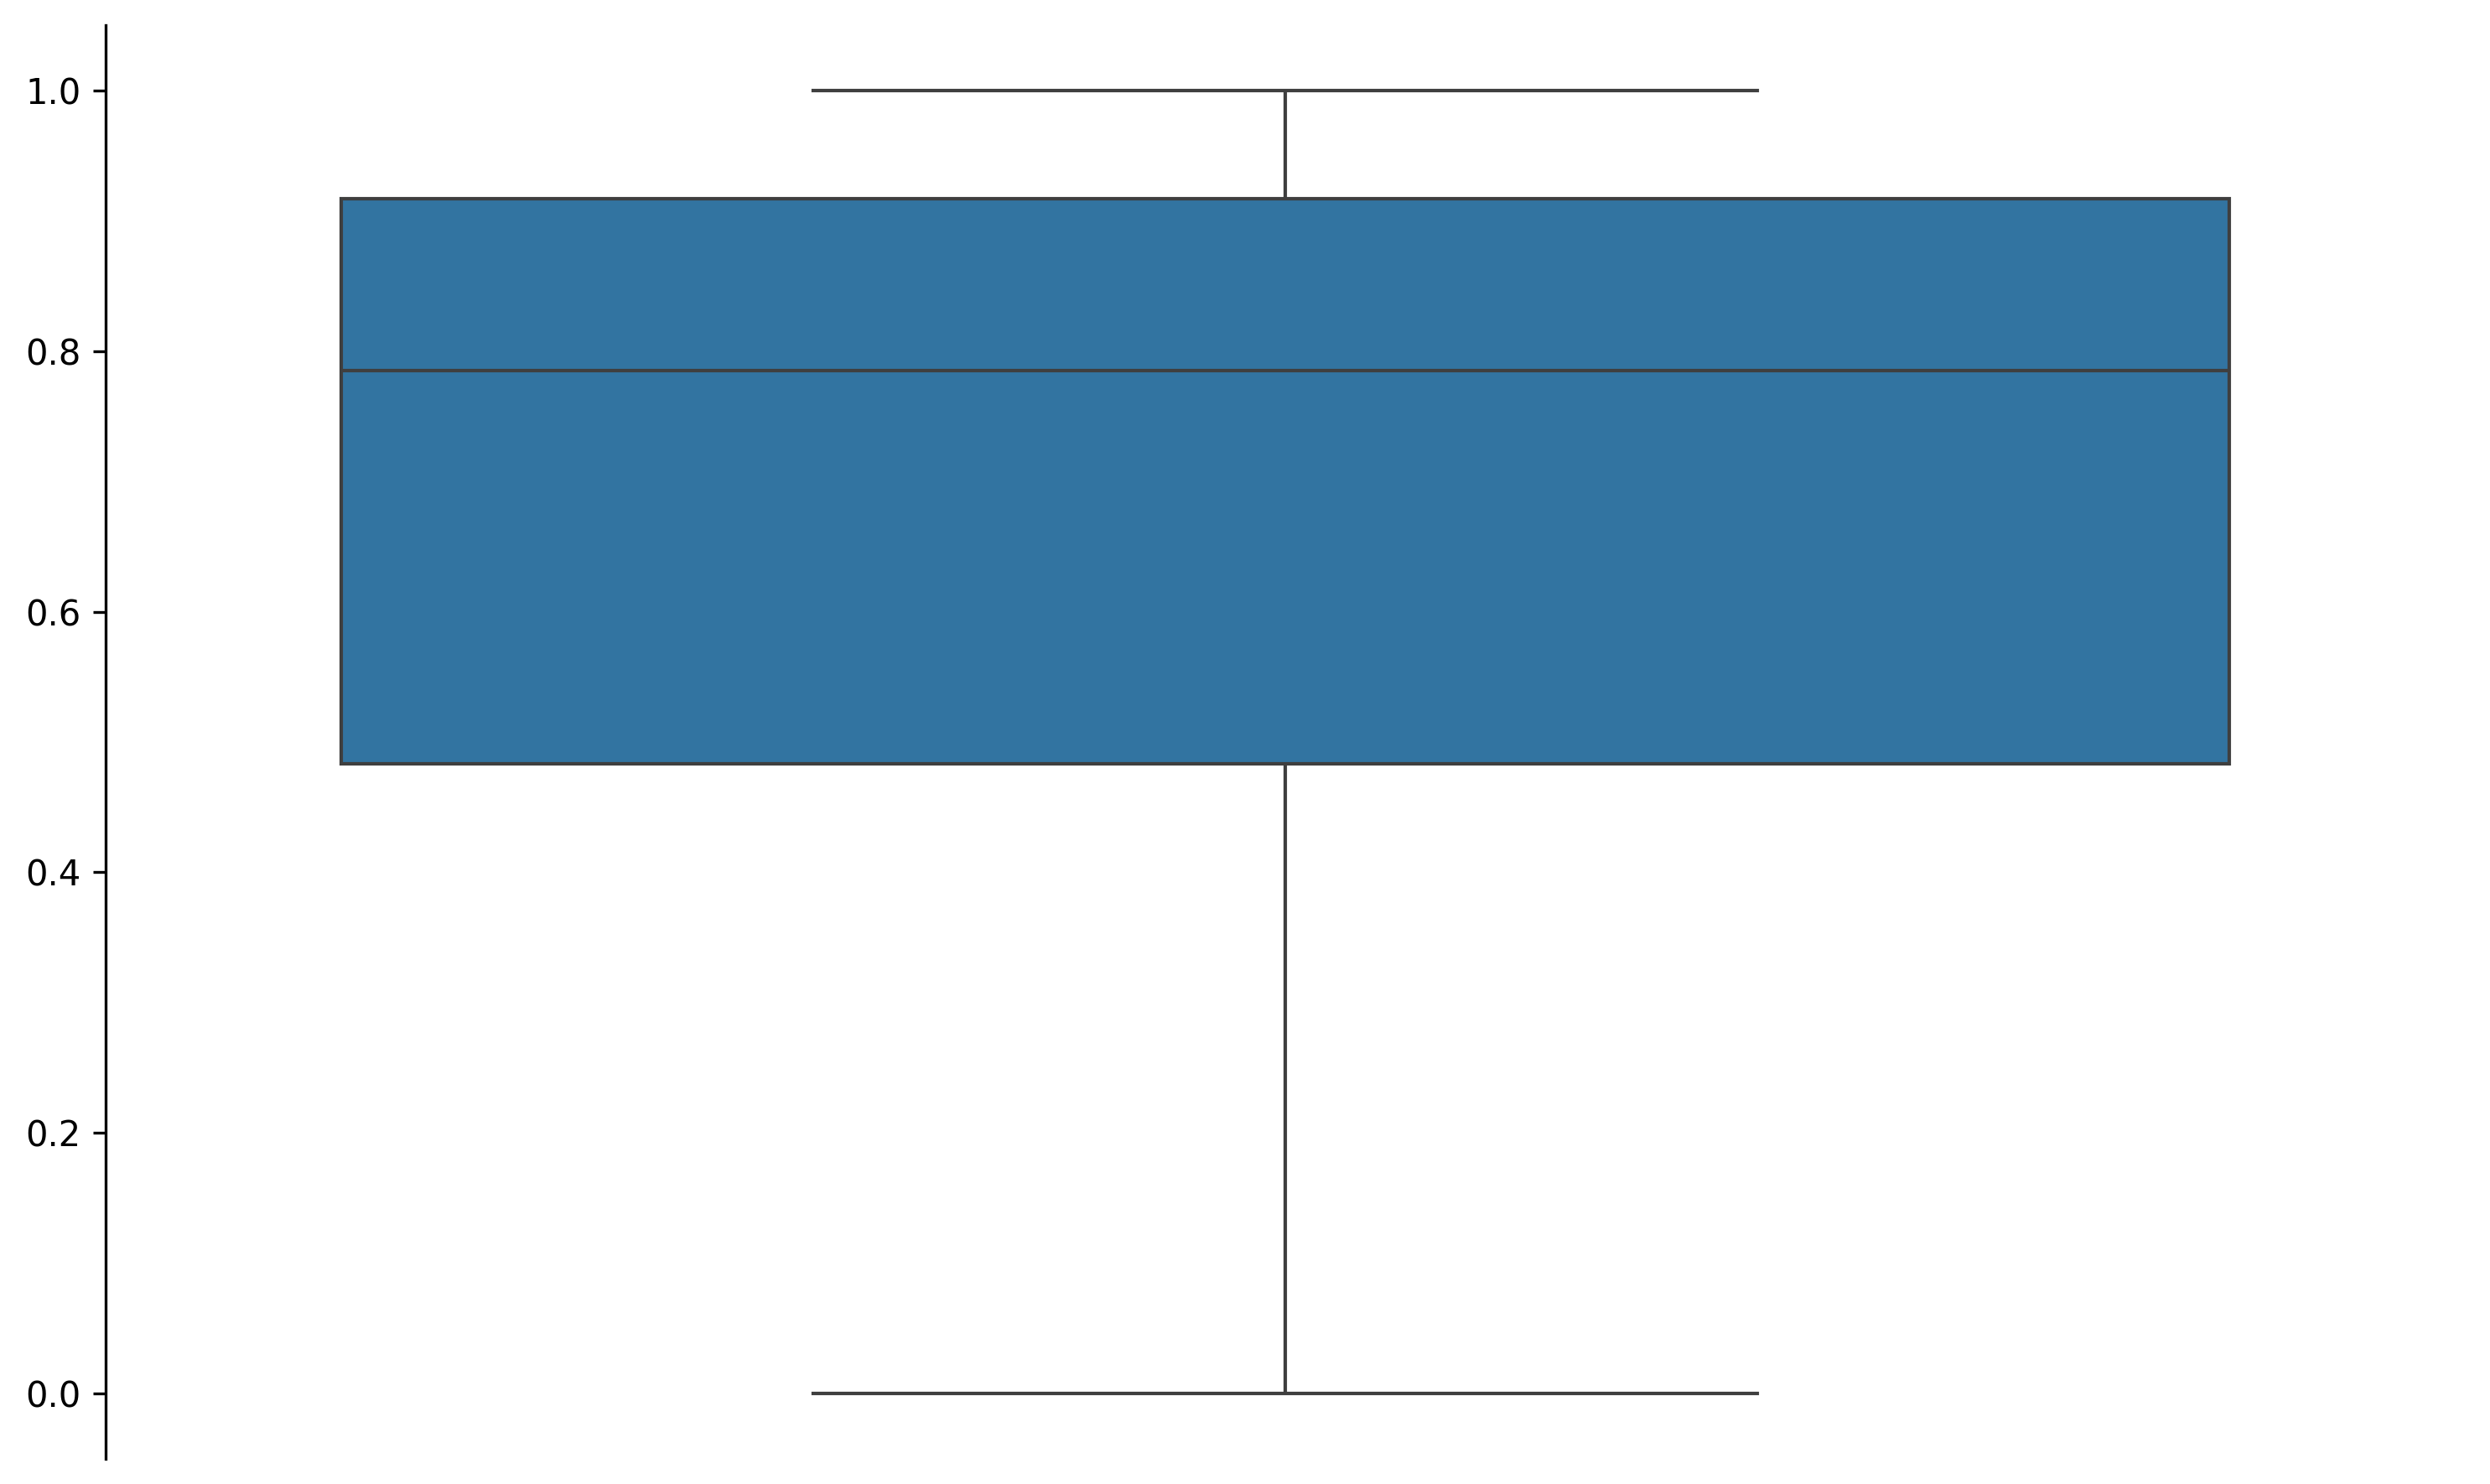
\includegraphics[width=1\linewidth]{figuras/egdi/boxplot_tci_global.png}
	\label{fig:boxplot_tci_global}
	\footnotesize{Fonte: baseado em \cite{ONU_EGDI_mapa}.}
\end{figure}

Os valores mínimo e máximo são, respectivamente, 0.0 e 1.0. O  valor médio é 0.79. Os 1º e 3º quartis são, respectivamente, 0.48 e 0.92.

\section{Coeficiente de correlação: EGDI, seus componentes e E-Participation comparados com o PIB \textit{per capita} PPC e os gastos públicos (\% do PIB)}

\textbf{COMENTARA QUI}

\begin{figure}[H]
	\centering
	\caption{Índice de democracia eleitoral}
	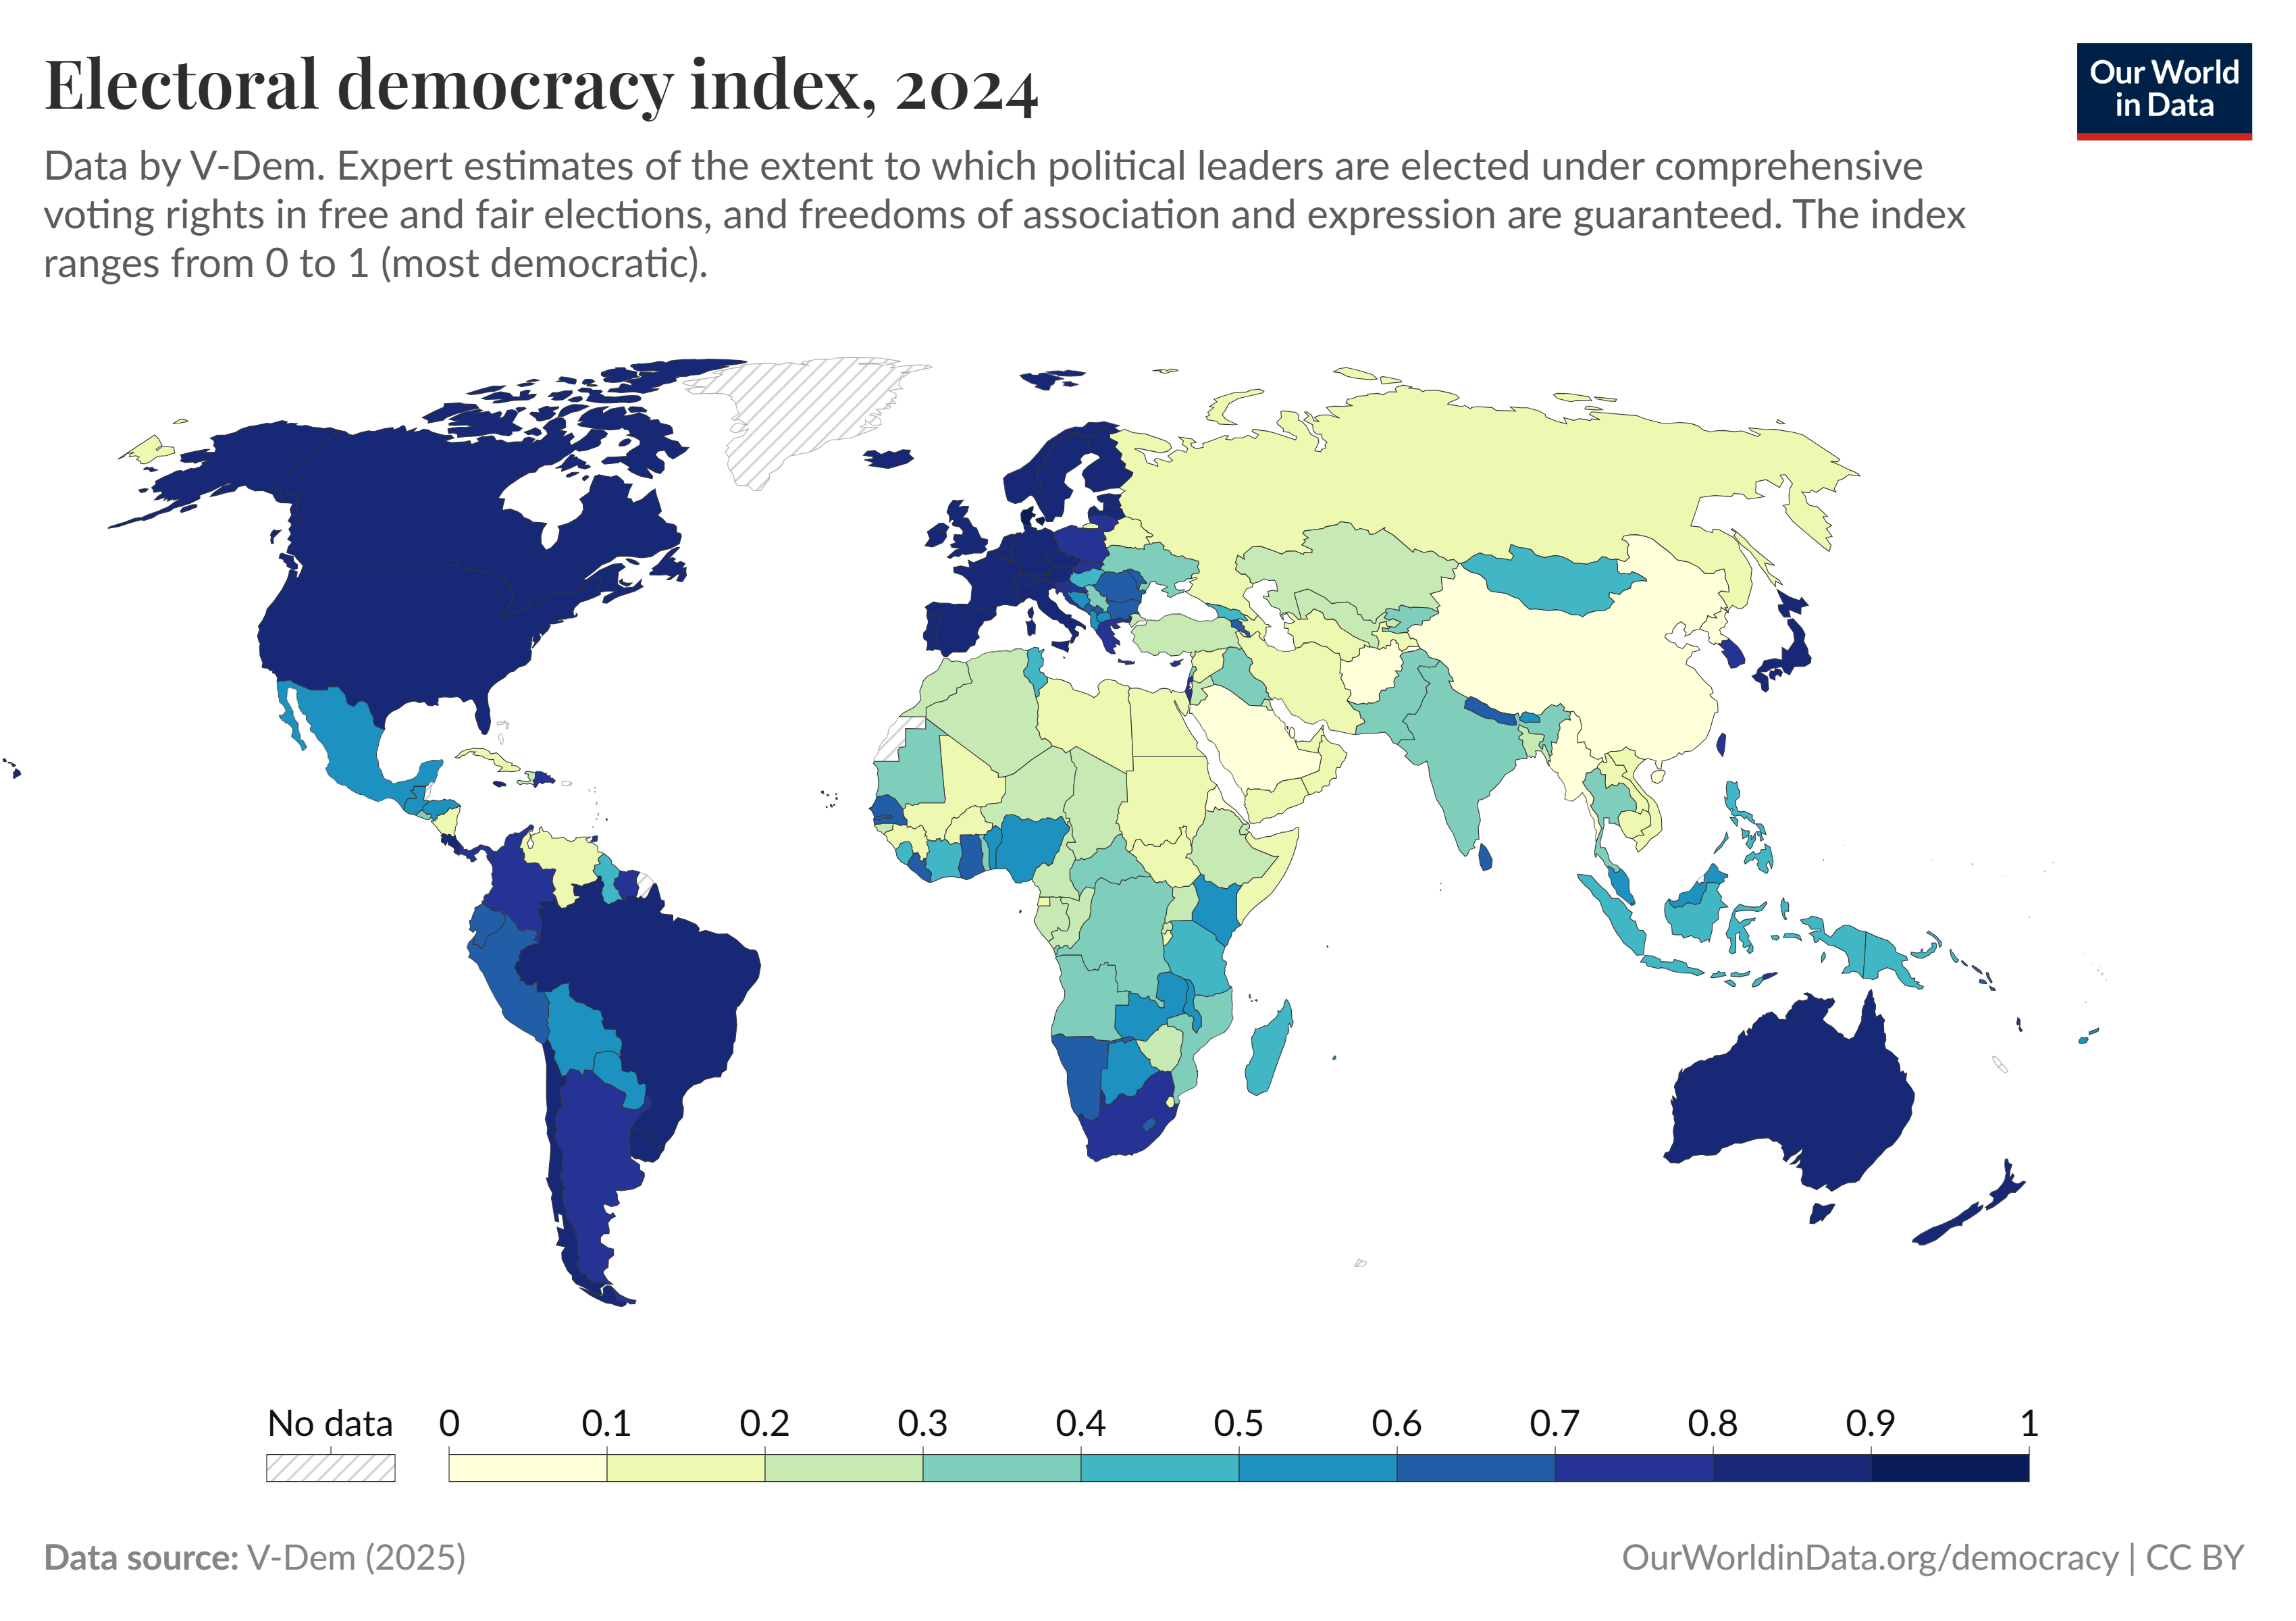
\includegraphics[width=1\linewidth]{figuras/democracia/electoral-democracy-index}
	\label{fig:electoral-democracy-index}
	\footnotesize{Fonte: \cite{electoral-democracy-index}.}
\end{figure}

\begin{figure}[H]
	\centering
	\caption{EGDI no mundo}
	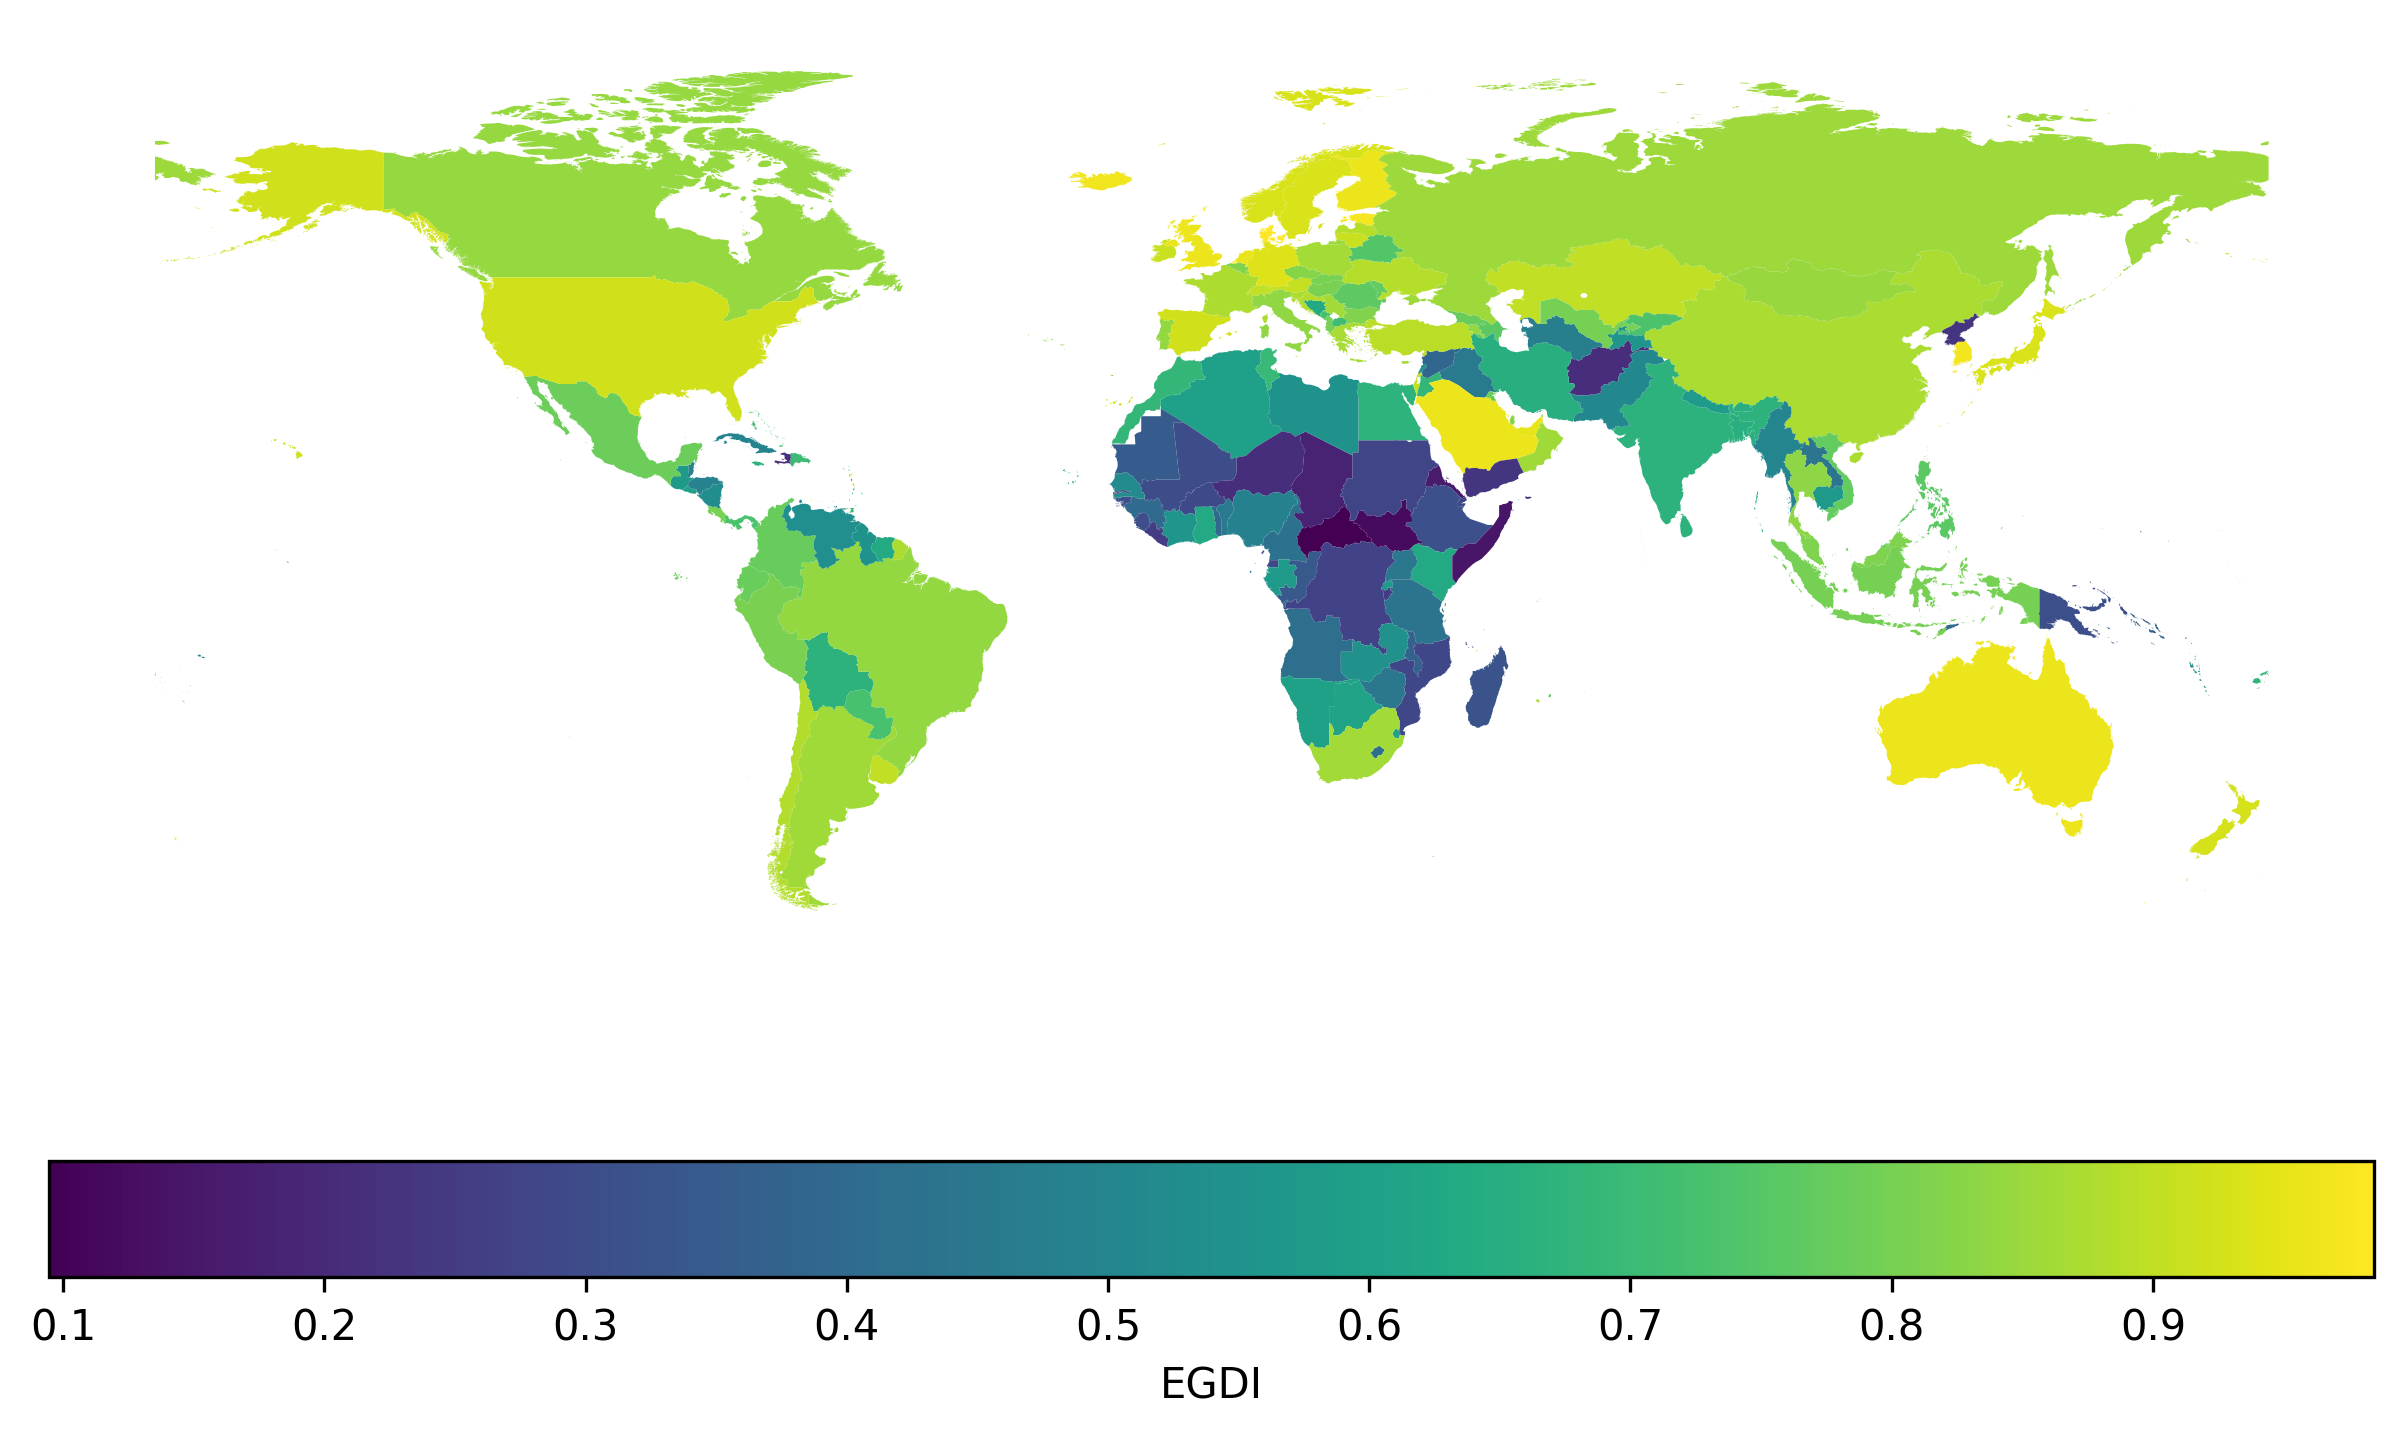
\includegraphics[width=1\linewidth]{figuras/egdi/mapa_coropleto_paises_egdi}
	\label{fig:mapa_coropleto_paises_egdi}
	\footnotesize{Fonte: \cite{ONU_EGDI_mapa}.}
\end{figure}

\begin{figure}[H]
	\centering
	\caption{Gastos públicos no mundo}
	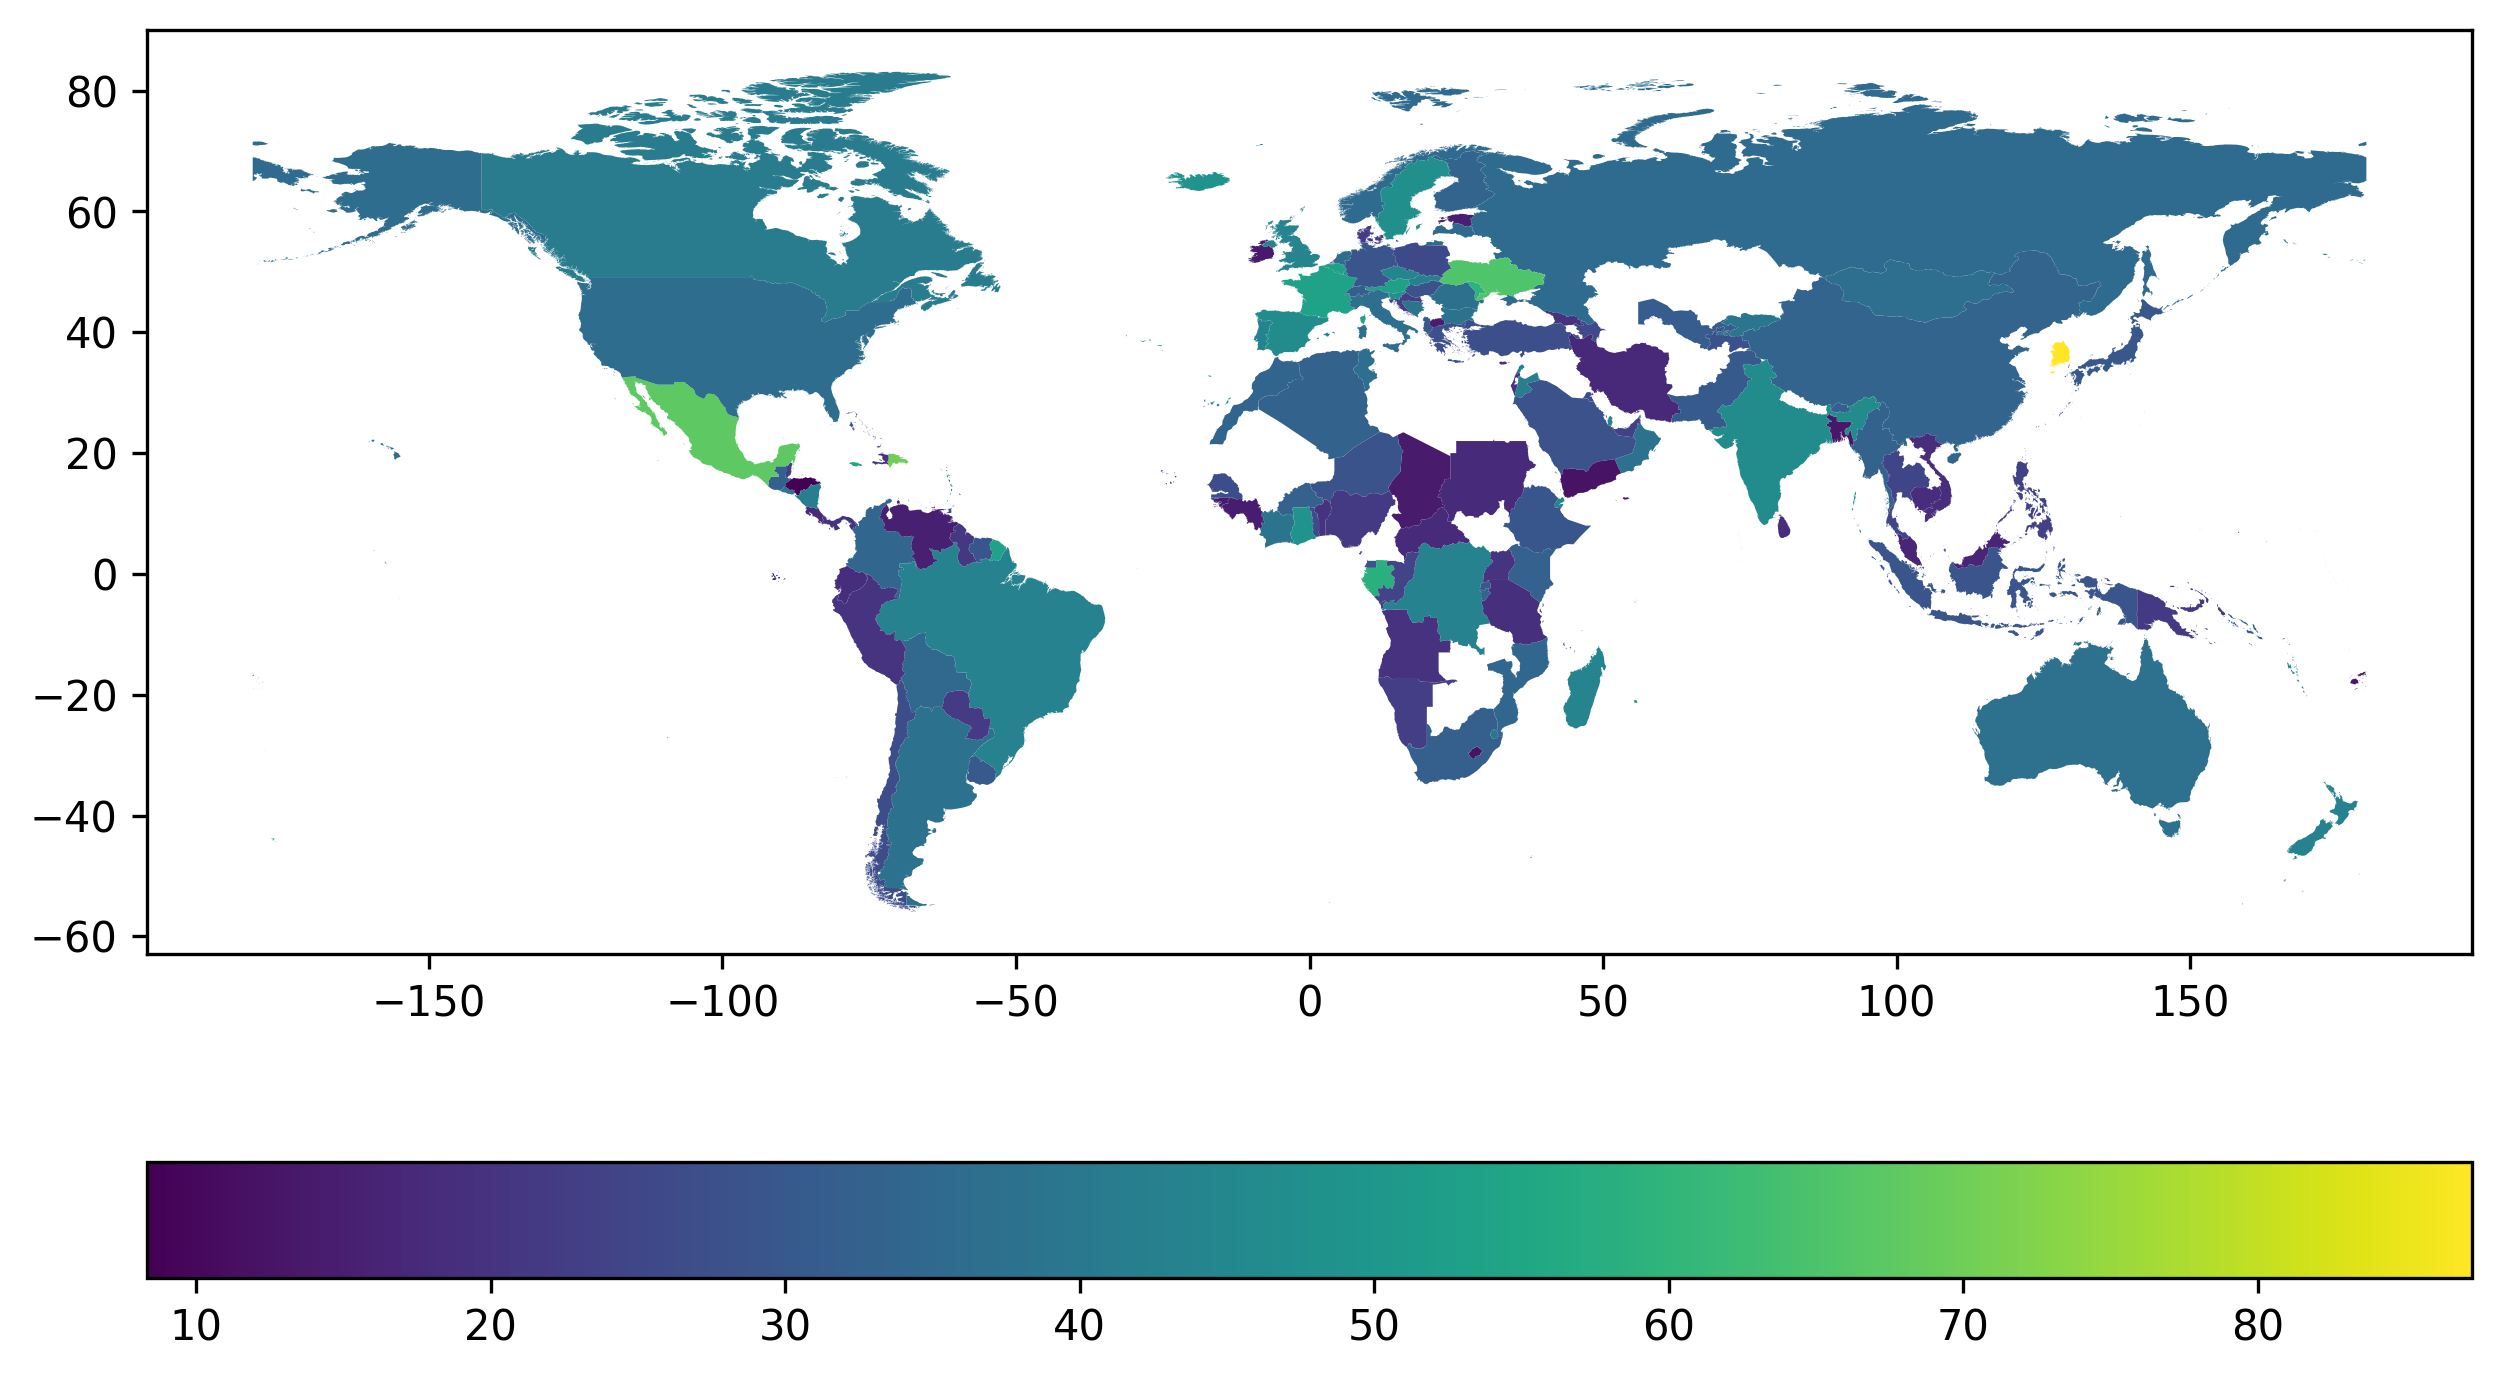
\includegraphics[width=1\linewidth]{figuras/government_spending/mapa_coropleto_paises_gastospublicos}
	\label{fig:mapa_coropleto_paises_gastospublicos}
	\footnotesize{Fonte: \cite{FMI_gov_expenditure}.}
\end{figure}

Com base nos parágrafos anteriores, um questionamento surgiu: qual é relação entre EGDI e \textbf{E-Participation Index} com o PIB \textit{per capita} e com os gastos públicos (\% do PIB). Para descobrir qual tipo de coeficiente de correlação usar, fez-se diagramas de dispersão. Caso haja linearidade, usar-se-á Pearson; caso contrário, Spearman.

\subsubsection{Análise do EGDI, seus componentes e E-Participation Index}

Analisar-se-á o aspecto geral usando o EGDI e o \textbf{E-Participation Index}, estudando como essas variáveis se comportam em diagramas de dispersão e coeficientes de correlação quando comparada com outras variáveis.

\subsubsection{EGDI e PIB \textit{per capita} PPC}

\begin{figure}[H]
	\centering
	\caption{Diagrama de Dispensao: EGDI e PIB \textit{per capita} PPC}
	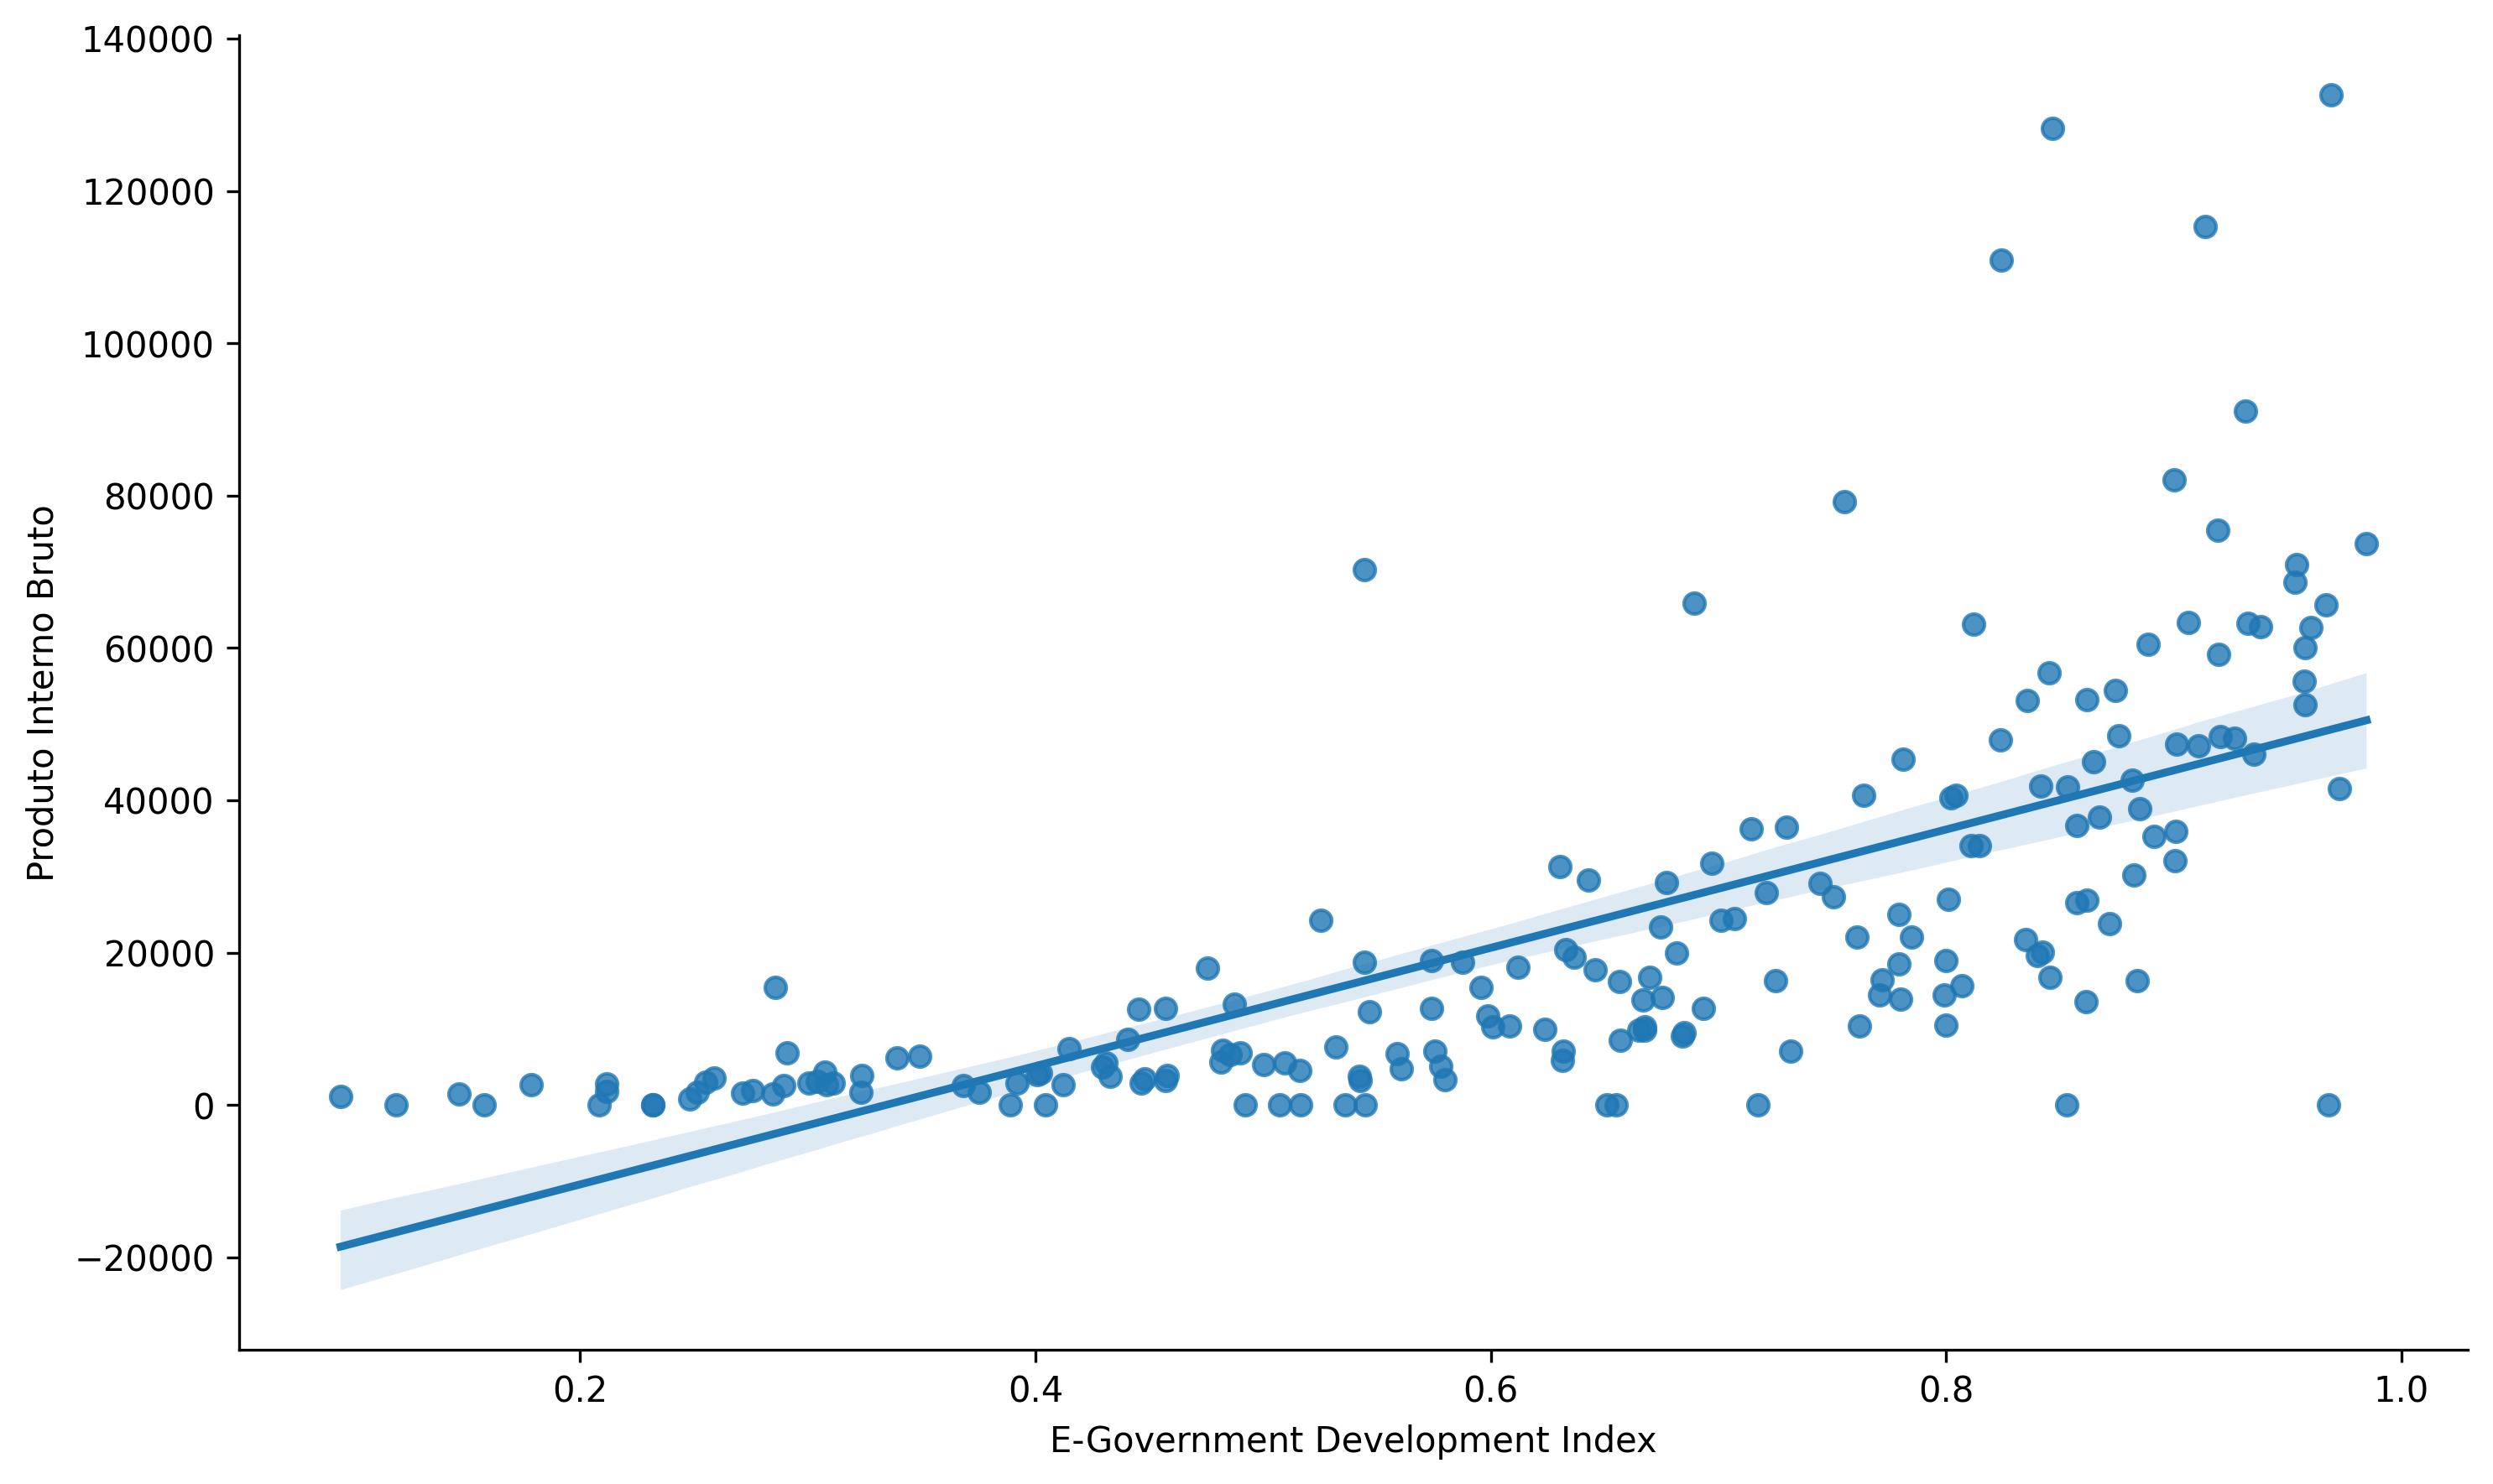
\includegraphics[width=1\linewidth]{figuras/egdi/dispensao_egov_pib}
	\label{fig:dispensao_egov_pib}
	\footnotesize{Fonte: \cite{ONU_EGDI} e \cite{WB_pib_per_capita_países}}
\end{figure}

Para compreender melhor o diagrama de dispersão, foi usado o coeficiente de correlação de Spearman. A sua escolha foi motivada pela grande presença de pontos extremos. O coeficiente de correlação encontrada foi 0.82. Devido ao coeficiente, os PIB \textit{per capita} PPC e o \textbf{E-Government Development Index} tendem a crescer juntos.

\cite{alisherovna2021whether} chegou a uma conclusão similar na figura \ref{fig:usmanova_egdi_gdp} a da figura \ref{fig:dispensao_egov_pib}, porém o autor adotou a taxa de crescimento do PIB ao invés do PIB \textit{per capita} PPC.

\begin{figure}[H]
	\centering
	\caption{Como os países se posicionam em relação ao EGDI de acordo com sua taxa de crescimento do PIB}
	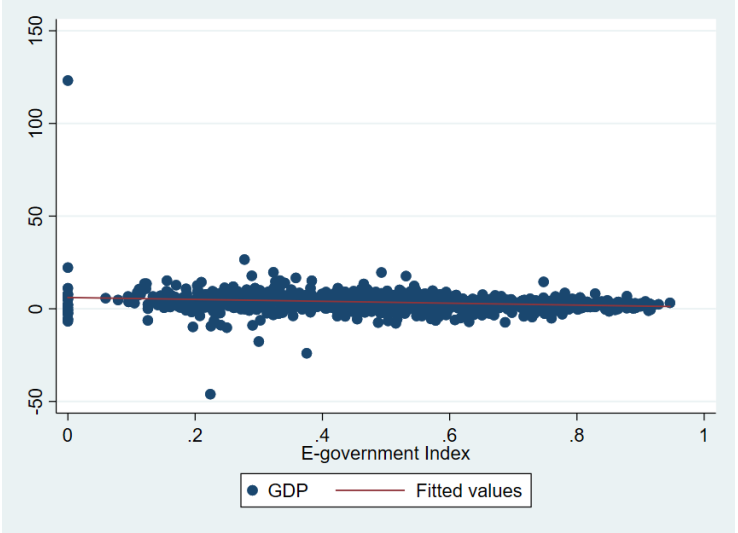
\includegraphics[width=1\linewidth]{figuras/egdi/usmanova_egdi_gdp}
	\label{fig:usmanova_egdi_gdp}
	\footnotesize{Fonte: \cite{alisherovna2021whether}}
\end{figure}

Embora a figura \ref{fig:usmanova_egdi_gdp} mostre menos pontos extremos do que a figura \ref{fig:dispensao_egov_pib}, percebe com o PIB, seja \textit{per capita} PPC ou sua taxa de crescimento tem forte correlação com o EGDI. 

Complementarmente, \cite{kumar2020cultural} descobriu que o desenvolvimento econômico, mensurado pelo PIB \textit{per capita}, significativamente e positivamente impulsiona o EGDI. 

\subsubsection{E-Participation Index e PIB \textit{per capita} PPC}

\begin{figure}[H]
	\centering
	\caption{Diagrama de Dispensao: E-Participation Index e PIB \textit{per capita} PPC}
	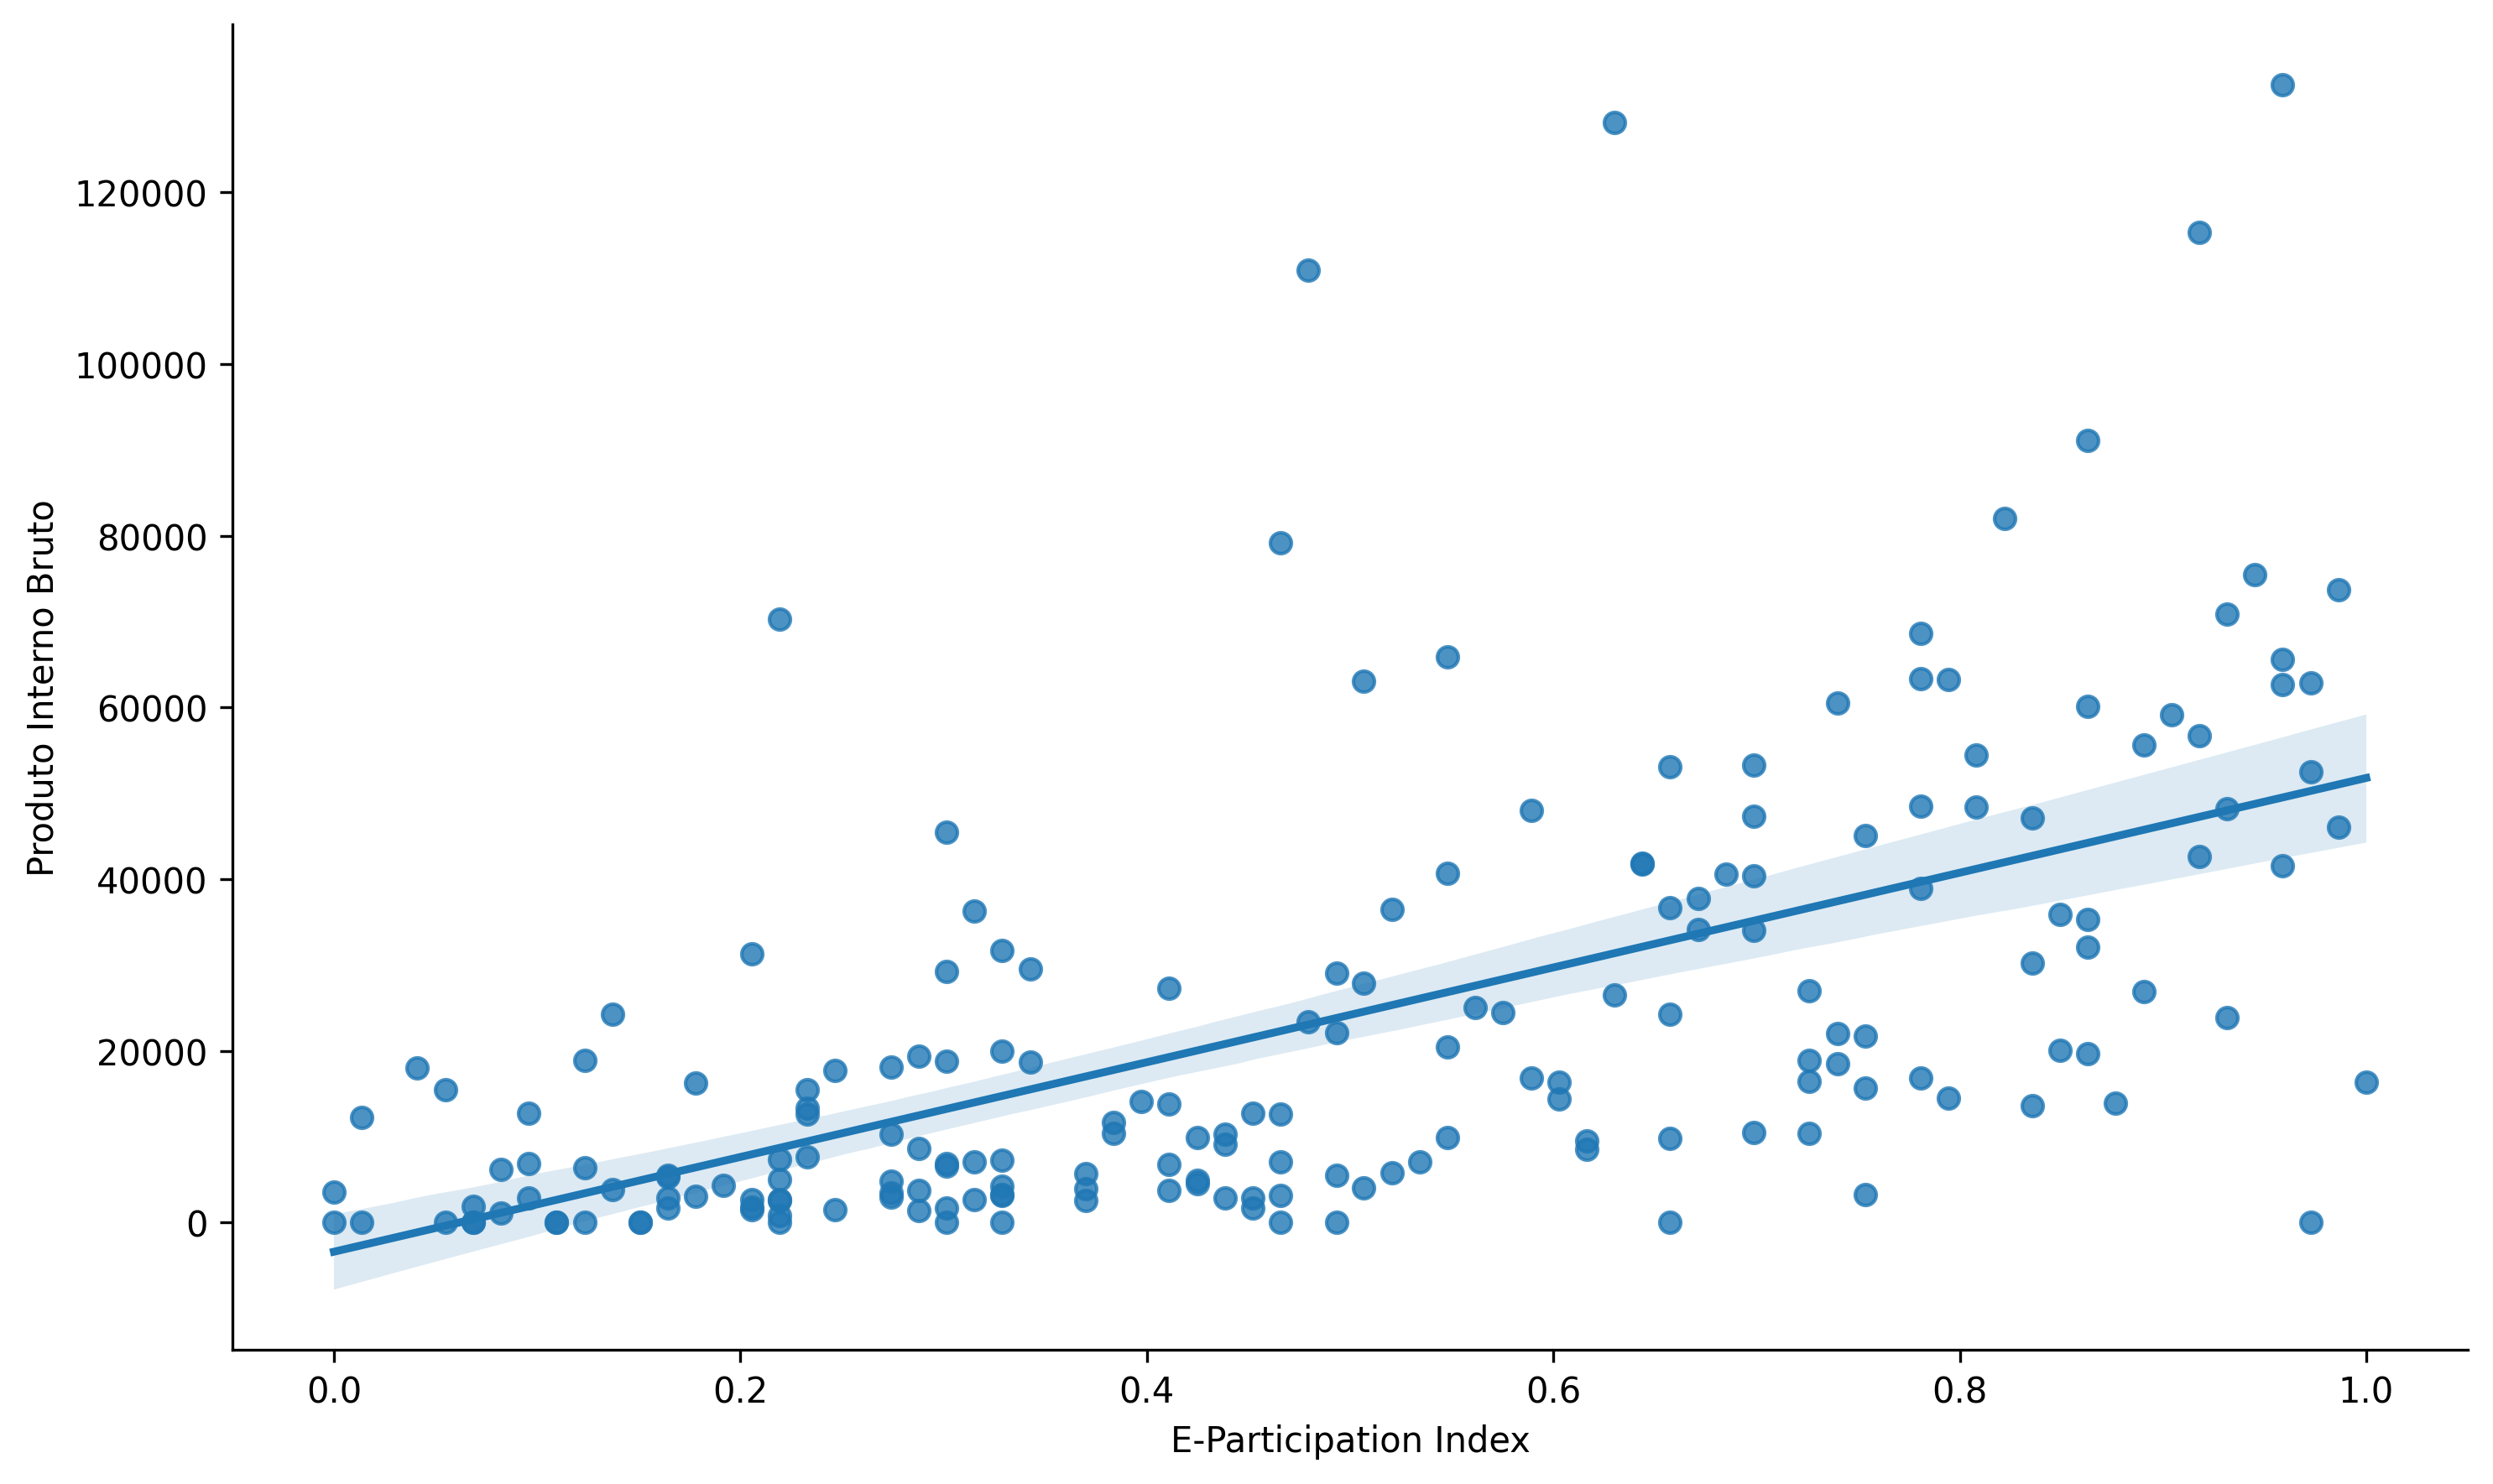
\includegraphics[width=1\linewidth]{figuras/egdi/dispensao_epart_pib}
	\label{fig:dispensao_epart_pib}
	\footnotesize{Fonte: \cite{ONU_EGDI_mapa} e \cite{WB_pib_per_capita_países}}
\end{figure}

Para compreender melhor o diagrama de dispersão, foi usado o coeficiente de correlação de Spearman. A sua escolha foi motivada pela grande presença de pontos extremos. O coeficiente de correlação encontrada foi 0.67. Devido ao coeficiente, os PIB \textit{per capita} PPC e o \textbf{E-Participation Index} tendem a crescer juntos.

\subsubsection{E-Government Development Index e gastos governamentais (\% do PIB)}

\begin{figure}[H]
	\centering
	\caption{Diagrama de Dispensao: E-Government Development Index e gastos governamentais (\% do PIB)}
	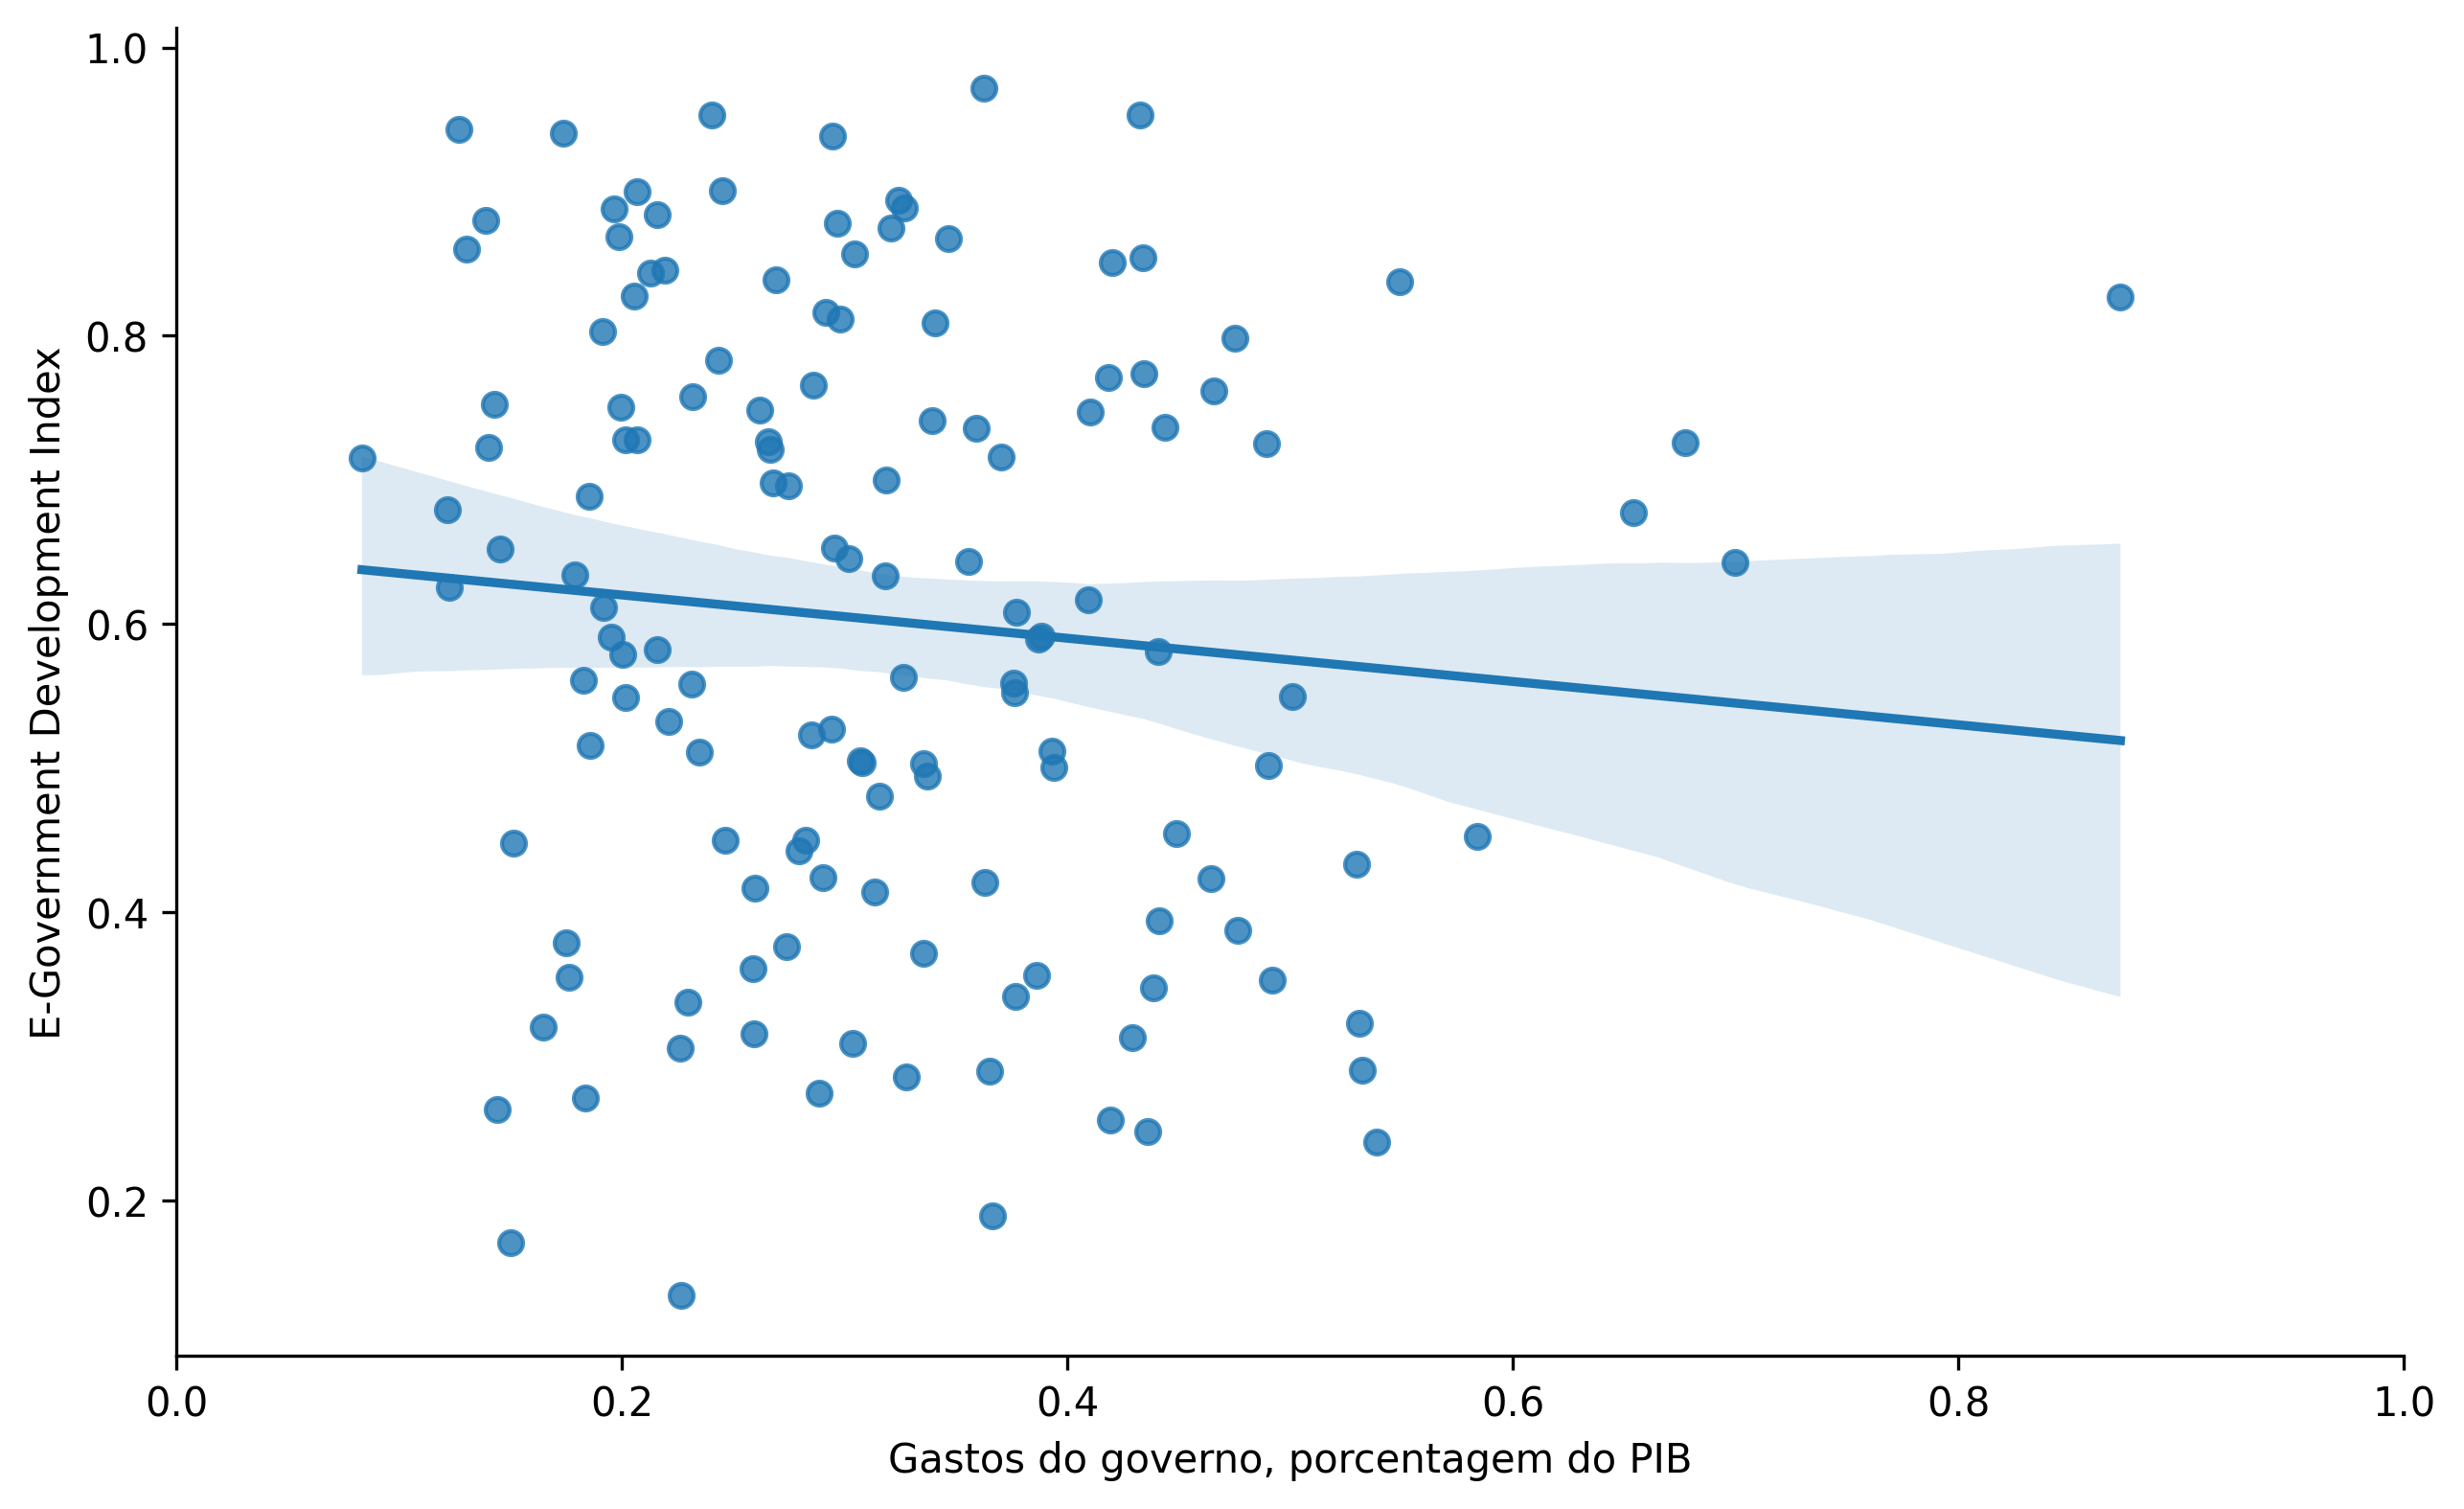
\includegraphics[width=1\linewidth]{figuras/egdi/dispersao_egov_govexpenditure}
	\label{fig:dispersao_egov_govexpenditure}
	\footnotesize{Fonte:baseado em \cite{ONU_EGDI_mapa} e \cite{FMI_gov_expenditure}}
\end{figure}

Para compreender melhor o diagrama de dispersão, foi usado o coeficiente de correlação de Spearman. A sua escolha foi motivada pela grande presença de pontos extremos. O coeficiente de correlação encontrada foi -0.13. O \textbf{E-Government Development Index} e os gastos públicos são variáveis independentes.

\subsubsection{E-Participation Index e gastos governamentais (\% do PIB)}

\begin{figure}[H]
	\centering
	\caption{Diagrama de Dispensao: E-Participation Index e gastos governamentais (\% do PIB)}
	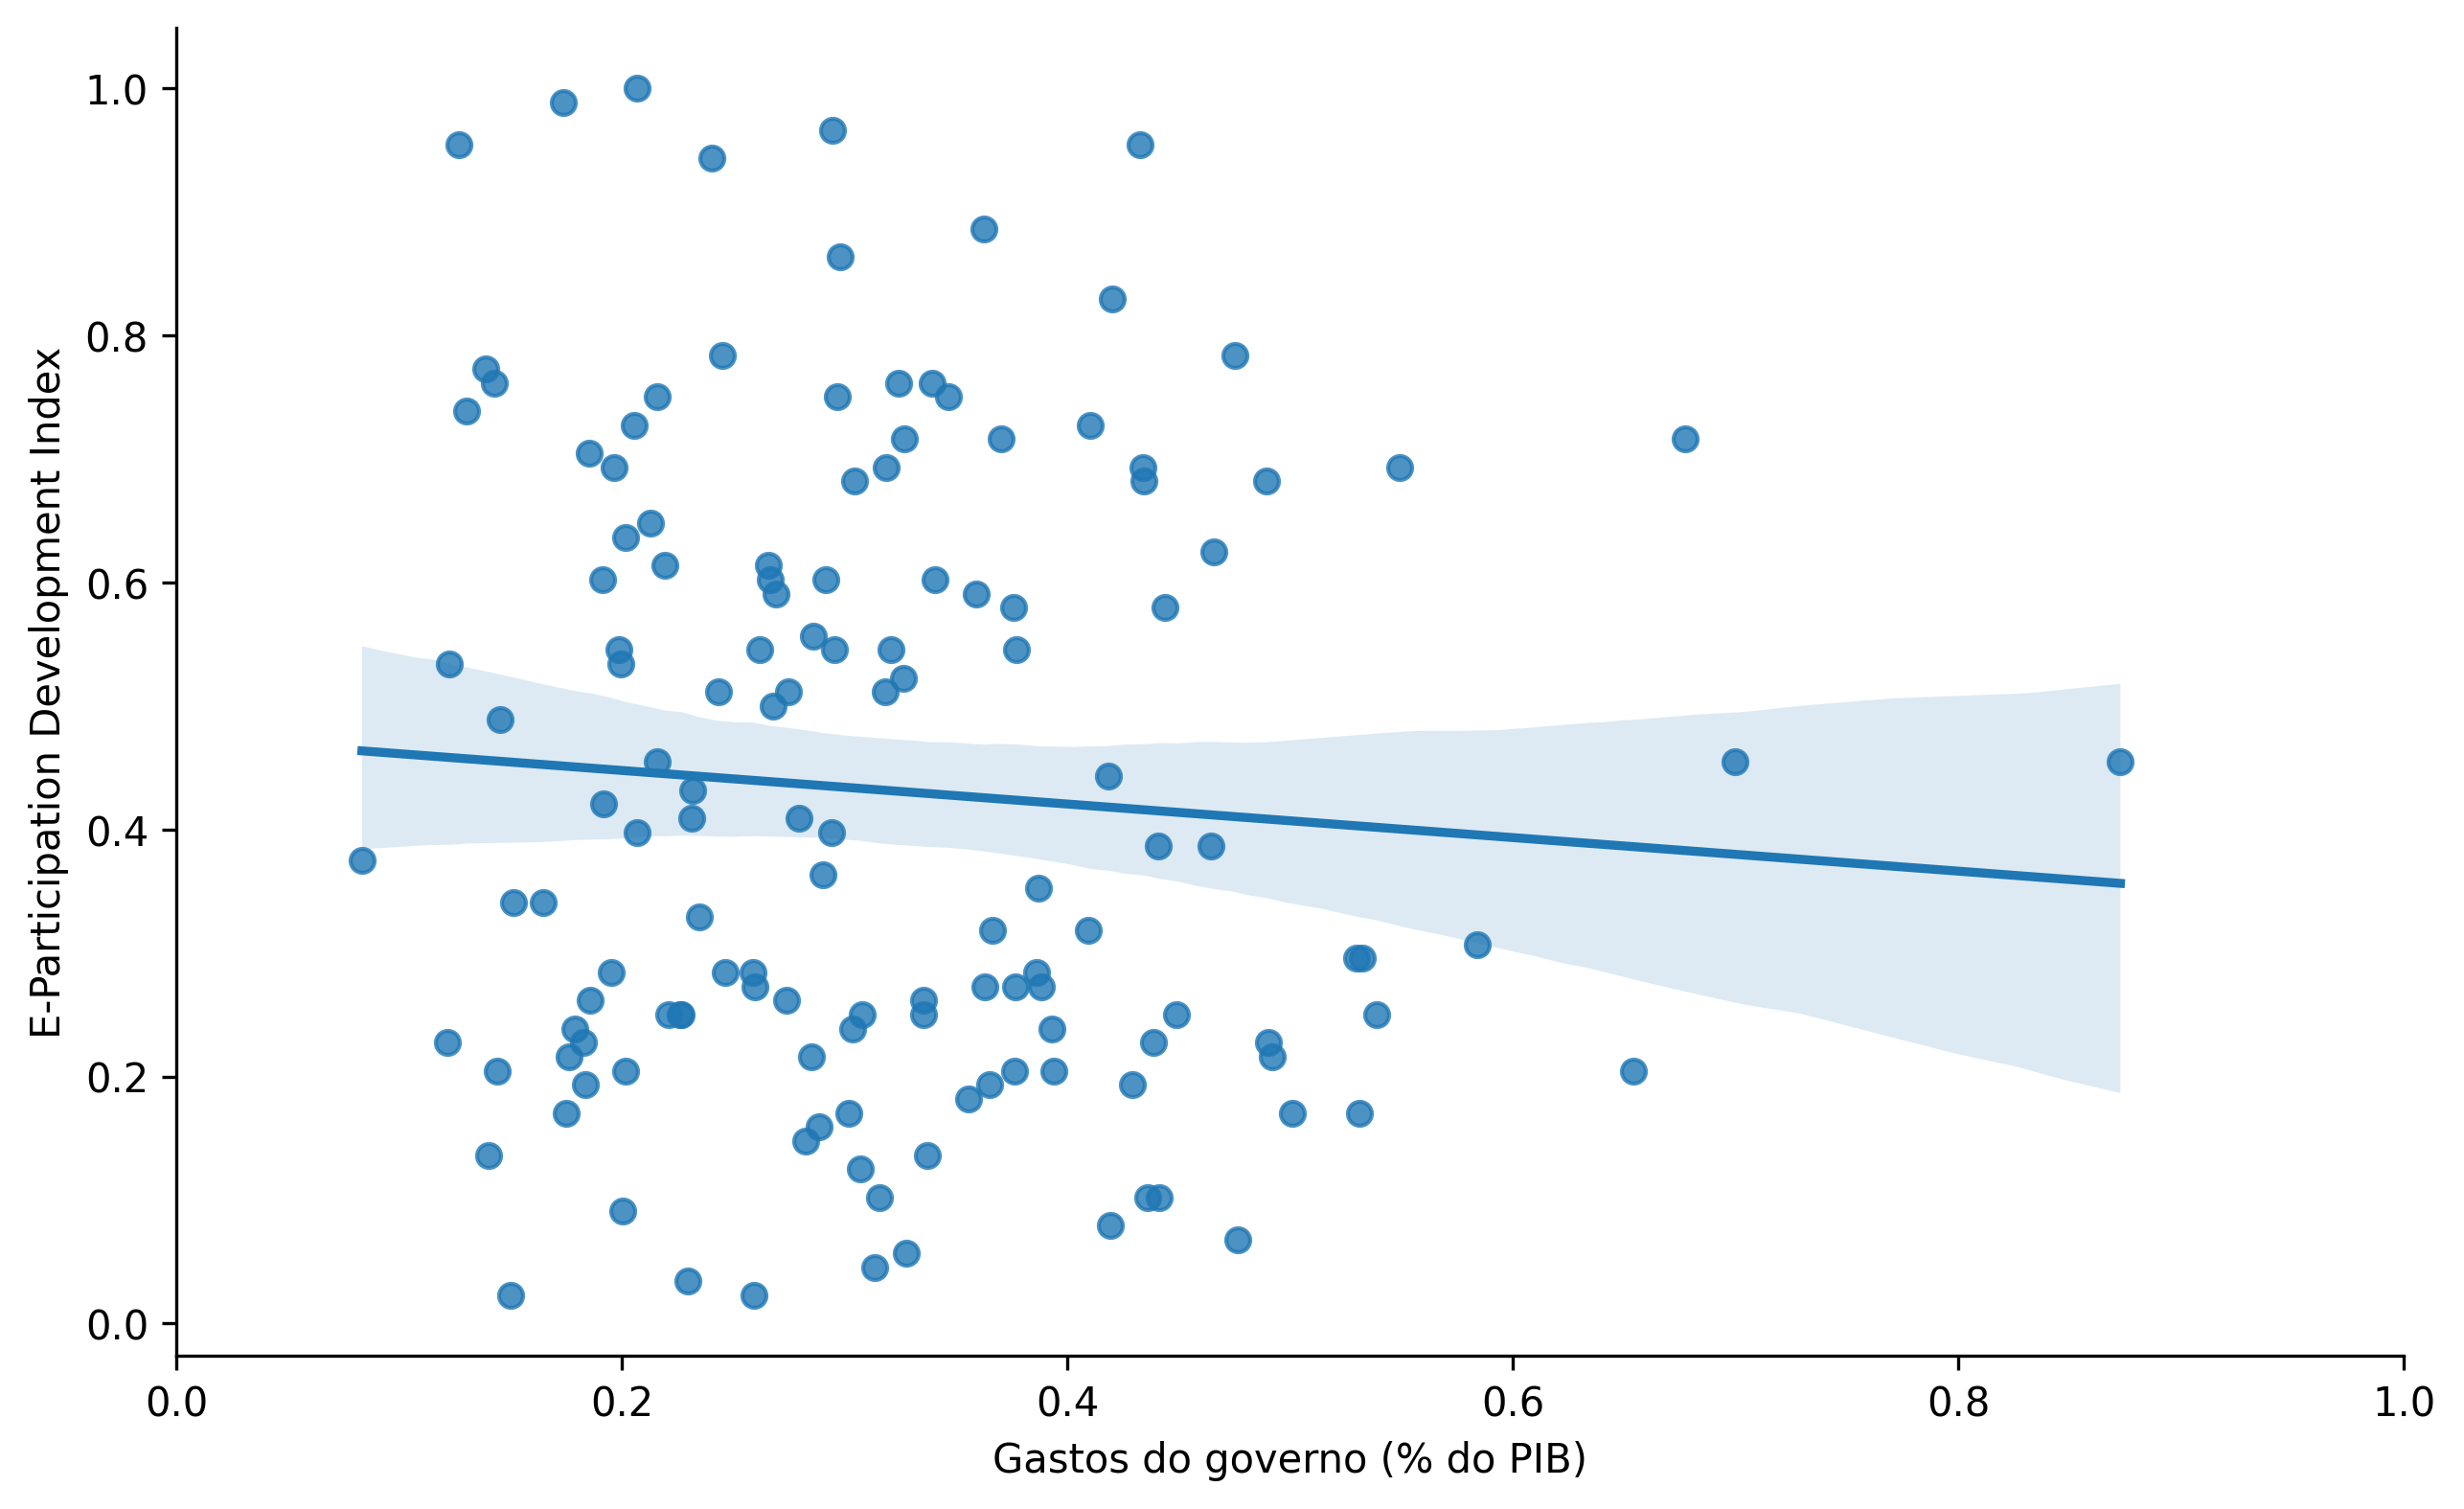
\includegraphics[width=1\linewidth]{figuras/egdi/dispersao_epart_govexpenditure}
	\label{fig:dispersao_epart_govexpenditure}
	\footnotesize{Fonte:baseado em \cite{ONU_EGDI_mapa} e \cite{FMI_gov_expenditure}}
\end{figure}

Para compreender melhor o diagrama de dispersão, foi usado o coeficiente de correlação de Spearman. A sua escolha foi motivada pela grande presença de pontos extremos. O coeficiente de correlação encontrada foi -0.07. O \textbf{E-Participation Index} e os gastos públicos são variáveis independentes.

\textbf{COMPARAR componentes do EGDI comparados com o PIB \textit{per capita} PPC e os gastos públicos (\% do PIB)}

\section{Dados do Brasil}

A figura \ref{fig:lineplot_egdi_brasil} mostra evolução do EGDI do Brasil desde 2003-2005 e 2008-2024 (bianualmente).

\begin{figure}[H]
	\centering
	\caption{Evolução do EGDI do Brasil (2003-2005, 2008-2024 bianualmente)}
	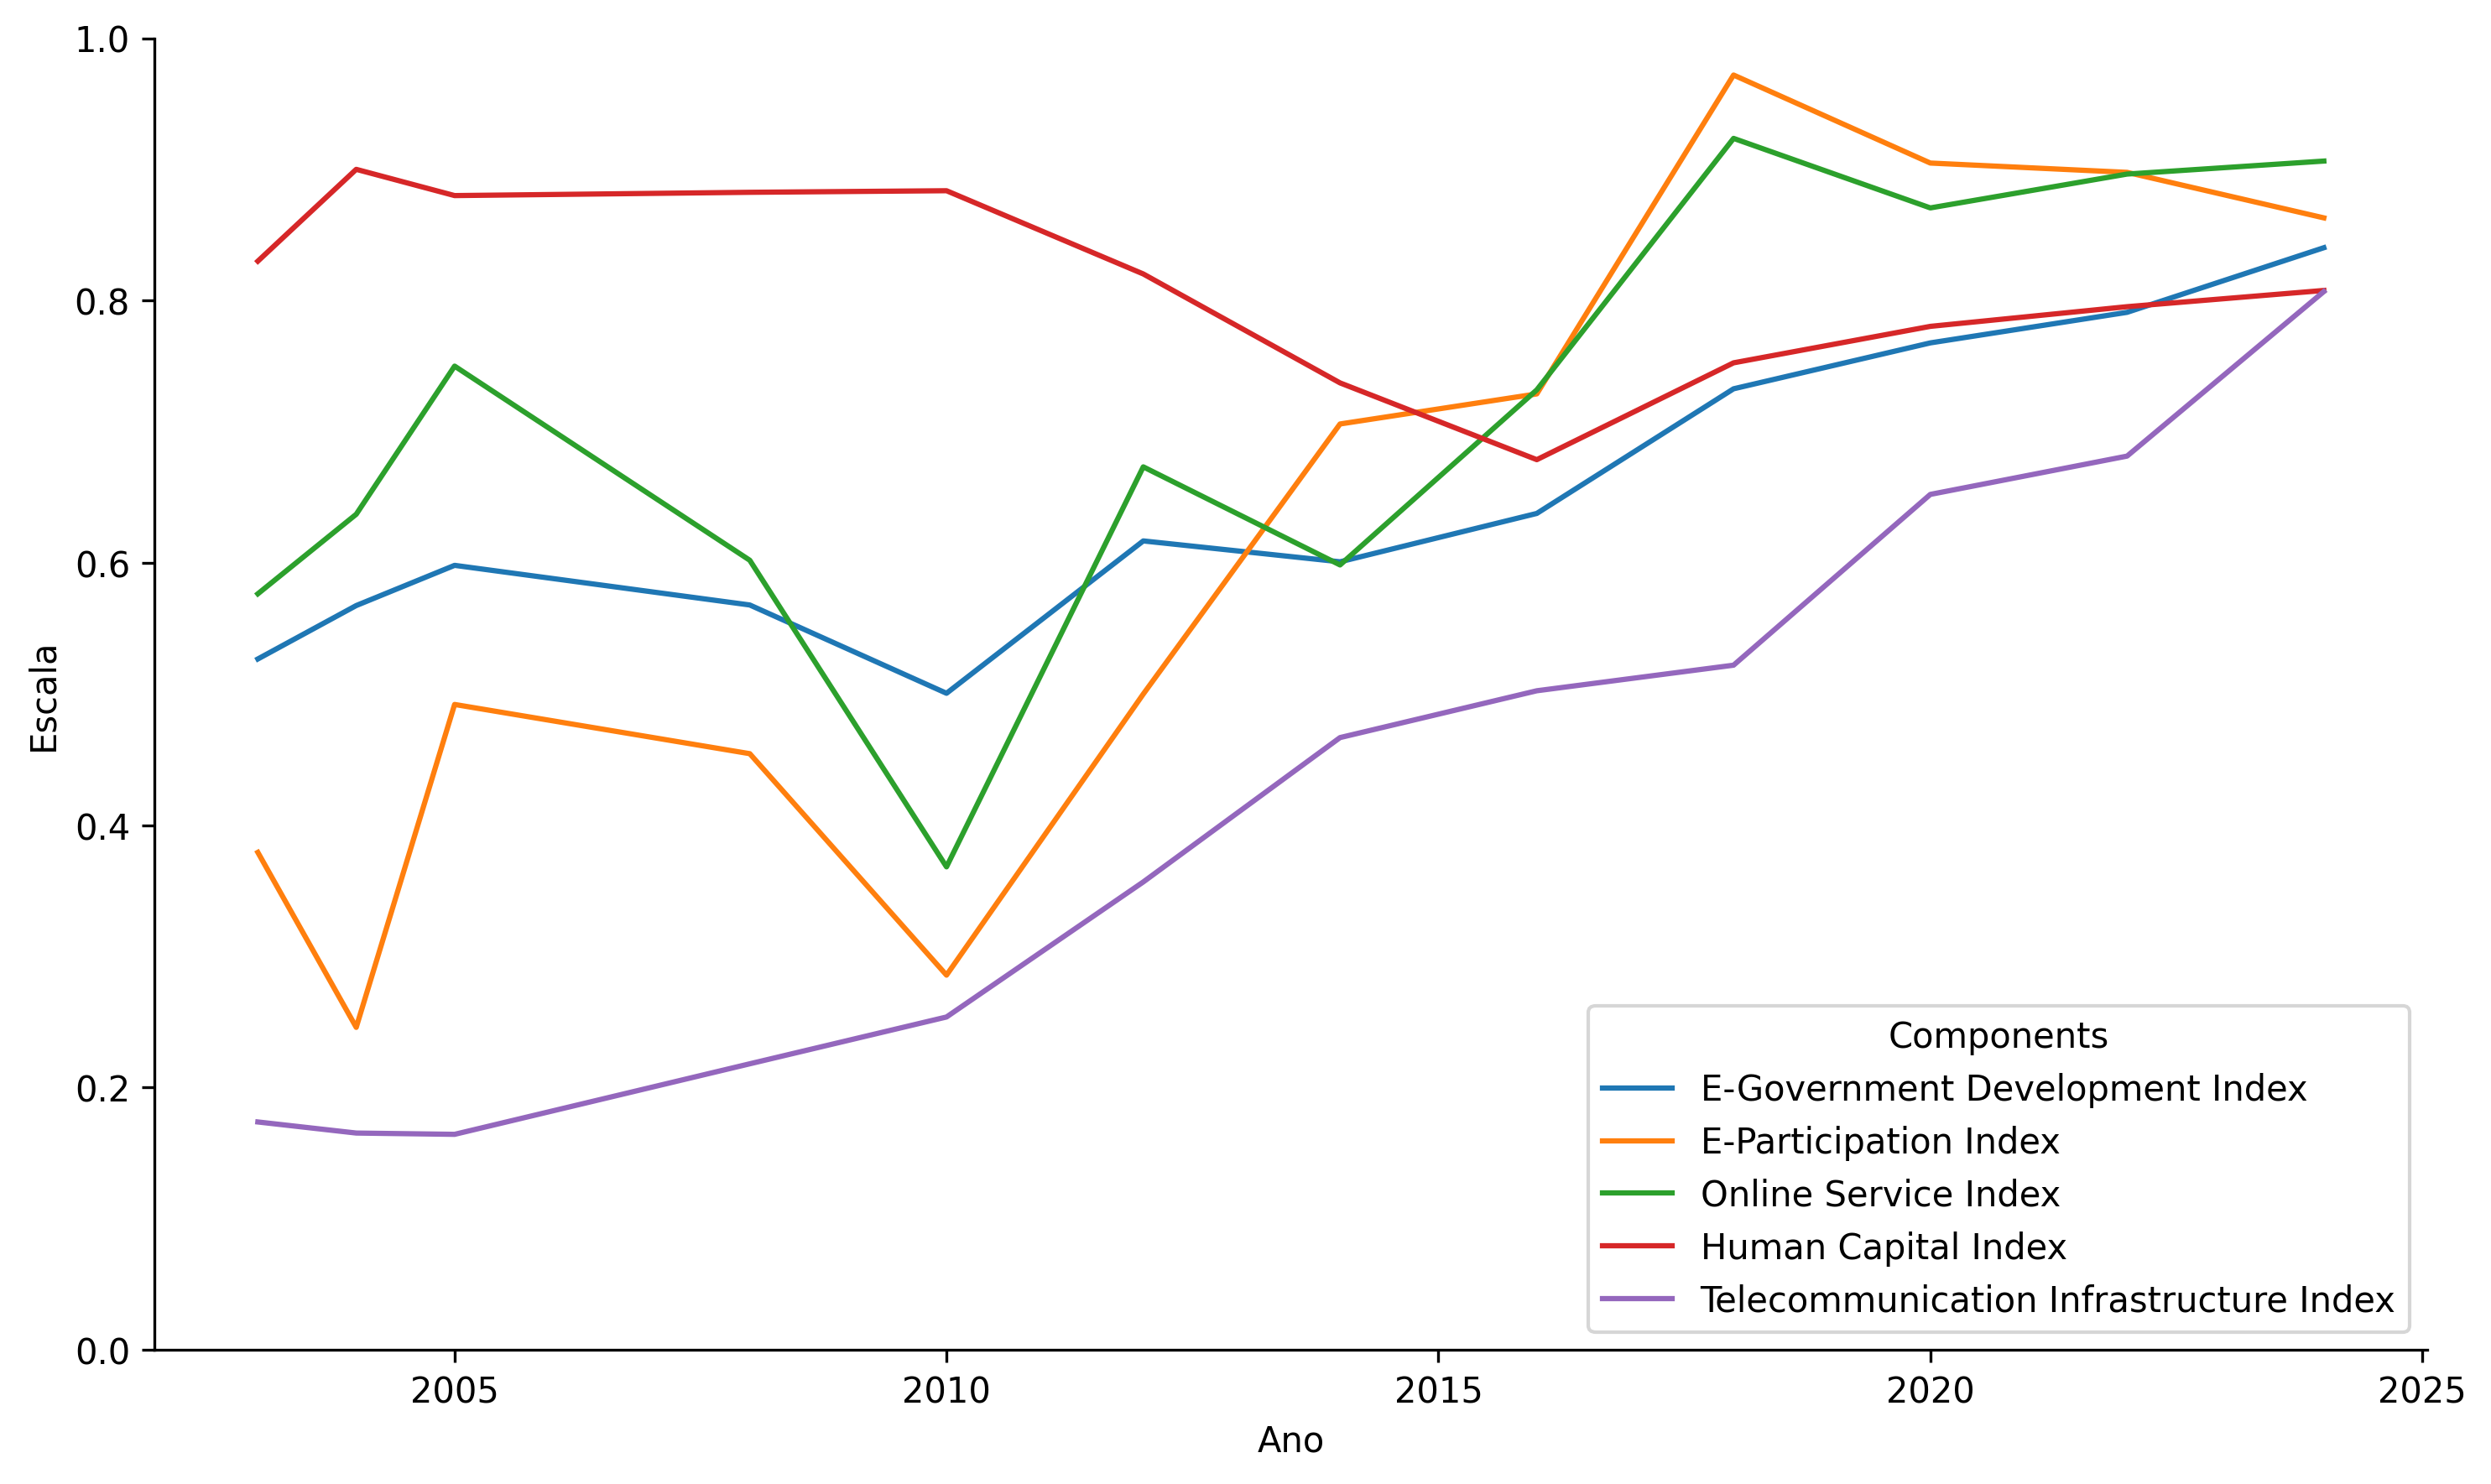
\includegraphics[width=1\linewidth]{figuras/egdi/lineplot_egdi_brasil.png}
	\label{fig:lineplot_egdi_brasil}
	\footnotesize{Fonte: baseado em \cite{ONU_EGDI_mapa}.}
\end{figure}

A maioria dos índices (\textbf{E-Government Development}, \textbf{Online Service},  \textbf{Human Capital} e, especialmente, o de  \textbf{Telecommunications Infrastructure}) apresenta uma tendência geral de crescimento ao longo do período, indicando uma melhoria na digitalização do governo e da sociedade brasileira.

Os  \textbf{E-Participation Index} e o \textbf{Online Service Index} mostram as maiores flutuações, com picos e quedas significativas em diferentes anos. Isso pode indicar variações nas políticas ou na implementação de serviços digitais e na participação cidadã.

\subsubsection{E-Government Development Index} O índice principal mostra um crescimento constante, mas gradual, partindo de cerca de 0.5 em 2003 e atingindo mais de 0.8 em 2024. Sua trajetória reflete a média dos outros componentes, indicando uma evolução geral da capacidade do governo de fornecer serviços online.

\subsubsection{E-Participation Index} Este índice é o mais volátil e o que apresenta o menor desempenho em grande parte do período. Ele tem um pico notável em 2005, seguido de uma queda e uma lenta recuperação. Isso sugere que a participação cidadã por meio de canais digitais é uma área que enfrenta desafios e flutuações, e seu desenvolvimento pode não ser tão linear quanto o de outros componentes.

\subsubsection{Online Service Index} Após um pico inicial, este índice apresenta uma queda acentuada por volta de 2010, seguido de uma recuperação e um novo pico em 2018. Sua trajetória é irregular, o que pode refletir desafios na oferta de serviços públicos online. No entanto, ele termina o período em um nível alto, próximo do Human Capital Index.

\subsubsection{Human Capital Index} Este índice mantém um nível consistentemente alto, geralmente entre 0.8 e 0.9, sendo o que mais se aproxima do valor máximo da escala. Apesar de algumas flutuações, ele demonstra que o Brasil possui um bom nível de capital humano para suportar o desenvolvimento do e-government, como educação e alfabetização digital.

\subsubsection{Telecommunication Infrastructure Index} Este é o índice com o crescimento mais notável e constante. Ele parte de um patamar baixo (abaixo de 0.2 em 2003) e alcança o maior valor entre todos os índices no final do período (próximo de 0.8 em 2024). Isso sugere um avanço significativo na infraestrutura digital do país, como a expansão de banda larga e redes de telecomunicações.

\subsection{Comparando as métricas do Brasil com a média internacional de 2024}

A figura \ref{fig:barplot_egdi_mediamundial_brasil} contém os valores do EGDI e seus componentes do Brasil e da média mundial de 2024.

\begin{figure}[H]
	\centering
	\caption{EGDI do Brasil e a média mundial em 2024}
	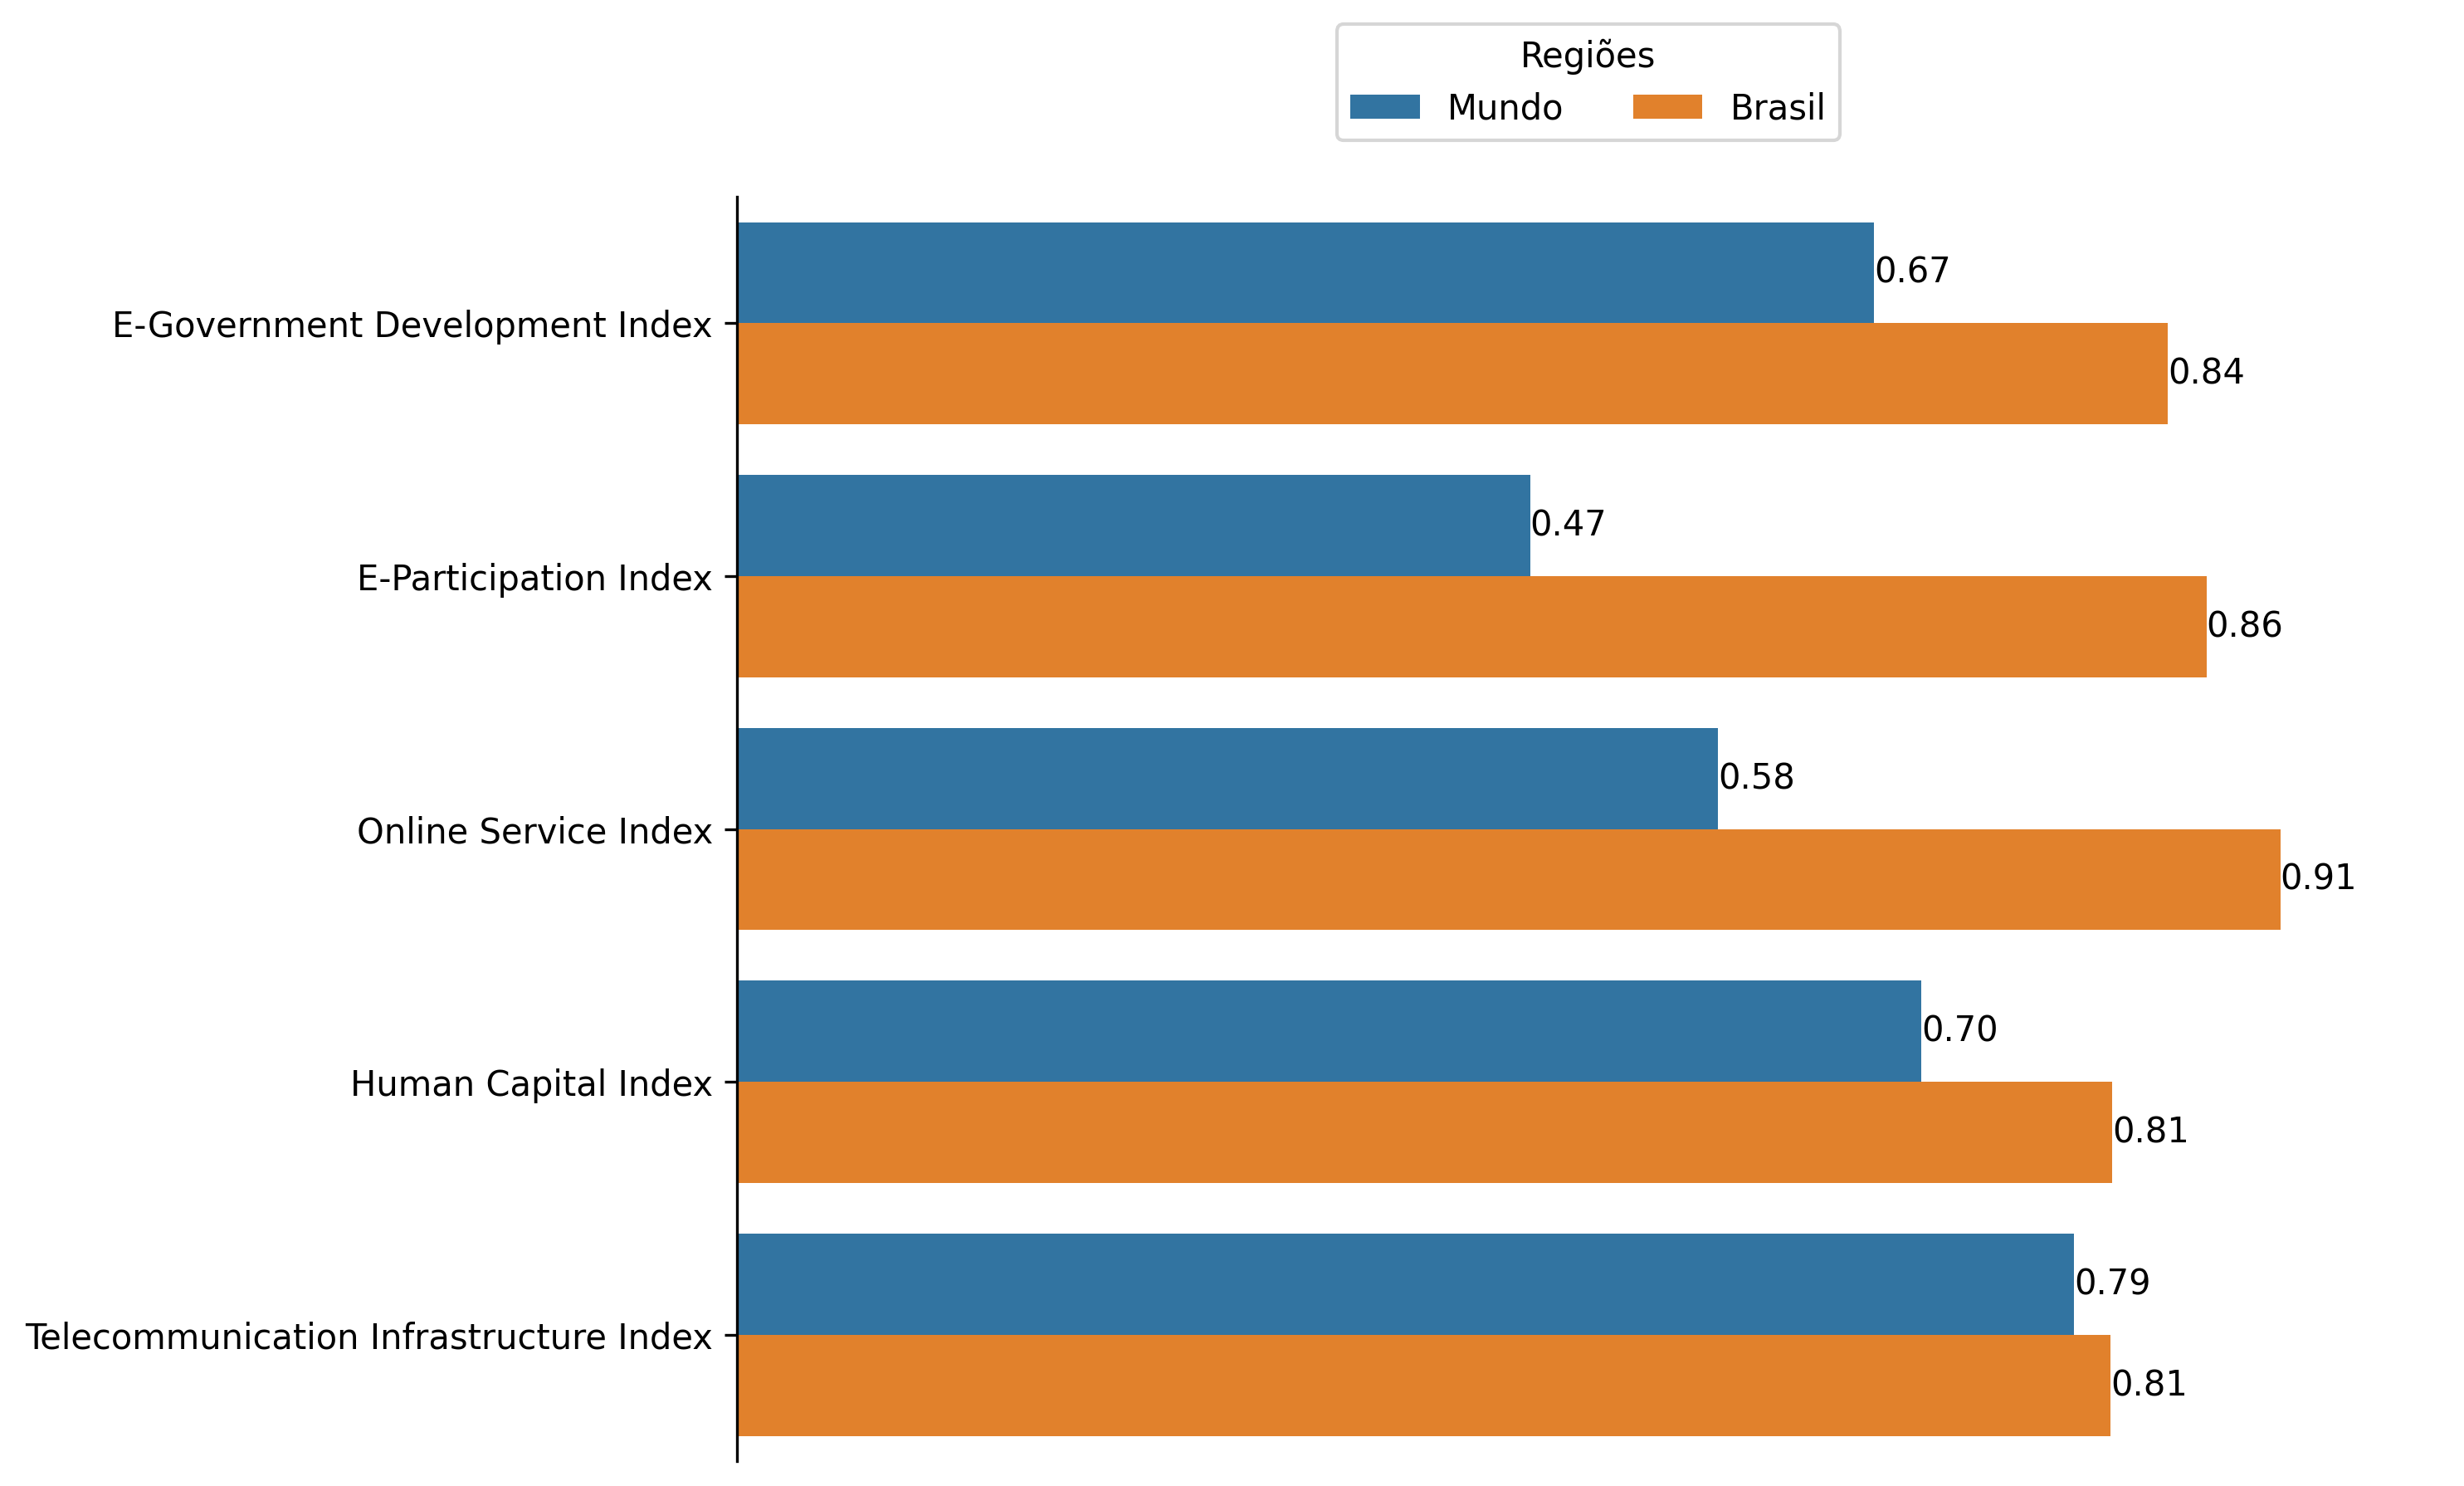
\includegraphics[width=1\linewidth]{figuras/egdi/barplot_egdi_mediamundial_brasil}
	\label{fig:barplot_egdi_mediamundial_brasil}
	\footnotesize{Fonte: baseado em \cite{ONU_EGDI_mapa}.}
\end{figure}

Nota-se como o Brasil está muito avançado em relação à média mundial.Os EGDI, \textbf{E-Participation Index}, \textbf{Online Service Index} e \textbf{Human Capital Index} foram os componentes que em mais o Brasil se detacou com 0.17, 0.29, 0.23 e 0.11 pontos acima da média mundial, respectivamente. O \textbf{Telecommunication Infrastructure Index} é o único componente em que a diferença entre à média mundial e o resultado apresentado pelo Brasil foi insiginificante (0.2 pontos de diferença).

